\documentclass[11pt]{article}

\usepackage[utf8]{inputenc}
\usepackage[T1]{fontenc}
\usepackage{lmodern}
\usepackage[margin=1in]{geometry}
\usepackage{graphicx}
\usepackage{booktabs}
\usepackage{amsmath}
\usepackage{xcolor}
\usepackage{caption}
\usepackage{float}
\usepackage{multirow}
\usepackage{microtype}
\usepackage{fancyhdr}
\usepackage{hyperref}

% --- typography: let TeX stretch a little harder before overflowing a margin
\emergencystretch=3em
\hbadness=4000
\tolerance=2000

% --- captions
\captionsetup{font=small, labelfont=bf, width=0.92\textwidth}

% --- running heads
\pagestyle{fancy}
\fancyhf{}
\fancyhead[L]{\small\nouppercase{\leftmark}}
\fancyhead[R]{\small\thepage}
\renewcommand{\headrulewidth}{0.4pt}
\fancypagestyle{plain}{\fancyhf{}\fancyhead[R]{\small\thepage}%
  \renewcommand{\headrulewidth}{0pt}}

% --- links: dark enough to read on paper
\definecolor{linknavy}{HTML}{16457A}
\hypersetup{
    colorlinks=true,
    linkcolor=linknavy,
    urlcolor=linknavy,
    citecolor=linknavy,
    pdftitle={Bus-Level Load Reconstruction --- Validation Results},
    pdfauthor={Rafael Leclerc},
    pdfsubject={Weather-dependent bus-level load reconstruction, ERCOT Coast to statewide Texas},
    pdfkeywords={load reconstruction, synthetic grid, ERCOT, ResStock, ComStock, LightGBM, Texas 7k},
    bookmarksnumbered=true,
    bookmarksopen=true
}

\title{Bus-Level Load Reconstruction --- Validation Results\\
\large From ERCOT Coast to Statewide Texas: Methodological Corrections, Model Choice,
Feature Engineering, and Validation Against All Eight ERCOT Weather Zones}
\author{Rafa\"el Leclerc}
\date{September 2026}

\begin{document}

\maketitle\vspace{-1.5em}

\begin{abstract}
\small
This report summarizes a series of methodological corrections and validation extensions
applied to the bus-level weather-dependent load reconstruction pipeline for the ERCOT
Coast zone (200-bus synthetic grid, IECC climate zone 2A), following review comments on
the draft paper. Two independent defects were identified and corrected: (1) a temporal
train/test leakage in the original random-split evaluation, and (2) a geography bug in
the weather station used to train and drive every model. On top of these fixes, a
head-to-head comparison of RandomForest, XGBoost, and LightGBM, and a feature-engineering
ablation study were carried out, all under a single consistent, leakage-free evaluation
protocol. A final validation pass compares every metric across all six pipeline versions
produced. The corrected pipeline improves the Pearson correlation against ERCOT Coast
actual load from 0.8818 to 0.9022, while providing an honest (non-inflated) picture of
per-archetype predictive accuracy --- though not every secondary validation metric improves
monotonically, a nuance discussed in Section~\ref{sec:validation}.

A second phase of work (Sections~\ref{sec:statewide}--\ref{sec:global}) extends the
corrected, feature-engineered LightGBM pipeline from the single Coast case study to all
five Texas IECC climate zones (254 counties, on a new, denser synthetic grid), for both
the residential and commercial stacks. This extension reuses the Coast
methodology as-is and is cross-checked against the already-validated Coast pipeline at
$r=0.9966$ (residential) and $r=0.9993$ (commercial). A stale RES\_SCALE/COM\_SCALE calibration was found and
fixed while doing this (Section~\ref{sec:recalibration}, resolving the first open item
from the previous phase), and a structural bus-coverage gap in the commercial
ZCTA-to-bus spatial join was identified but left unresolved
(Section~\ref{sec:statewide}). A second, independent, out-of-Coast validation against real
ERCOT load was obtained for IECC zone 3B (West Texas/Permian) against ERCOT's own WEST and
FAR WEST weather zones ($r=0.71$, materially weaker than Coast, most likely because West
Texas load carries a larger and more weather-independent industrial share that this
pipeline does not model at all). Finally, summing all five zones and comparing against
ERCOT's true statewide total load yields the strongest system-level correlation obtained
in this project so far ($r=0.9221$ uncalibrated, $r=0.9231$ with Coast's calibration
applied statewide) --- a genuinely new, global result, though at that stage still without
an independent statewide calibration or any industrial model outside Coast.

A third phase (Sections~\ref{sec:areasplit}--\ref{sec:zonecal}) removes the three
remaining structural limitations. The winner-takes-all spatial join underlying every
earlier number --- one census tract or ZIP-code area to one bus --- is replaced by an
area-split allocation over the full 6{,}717-bus grid, conserving 100\% of Texas housing
units while raising the share of load-carrying buses receiving commercial load from
20.1\% to 96.1\% and lifting bus-level rank agreement with the grid case's own per-bus
load from $\rho=0.133$ to $0.475$ --- an improvement invisible to every zone-aggregate
metric, which is itself an argument for reporting a bus-level statistic. Validation is
then extended to \emph{all eight} ERCOT weather zones via a per-bus assignment carried
by the grid model itself, rather than the GIS shapefiles previously assumed necessary;
the zone-3B finding is sharpened, locating the weakness specifically in West Texas
($r=0.629$ for FAR WEST) rather than in dry climates generally. Calibration is finally
refitted per zone with a \emph{data-driven} industrial constant, scored out-of-sample:
Coast's factors do not transfer (applied statewide with no industrial term they already
reach 105\% of ERCOT's true peak), the refitted residential factors collapse from
1.6--1.9 to 1.07--1.36, and the missing weather-insensitive load is quantified at
18{,}079\,MW statewide, or 24.7\% of system peak.
\end{abstract}

\vspace{1.5em}
\tableofcontents
\listoffigures
\listoftables
\clearpage

\section{Context}

The goal of this project is to reproduce and then improve on the bus-level,
weather-dependent load reconstruction framework described in Kang, Baembitov,
Safdarian, Snodgrass, and Overbye, applied to the ERCOT Coast weather zone (a 200-bus
synthetic grid, IECC climate zone 2A, covering the Houston/Galveston area). The
pipeline combines NREL ResStock/ComStock building archetype simulations, Census and
County Business Patterns (CBP) data, and weather-driven machine learning models to
reconstruct hourly, bus-level electricity load, which is then validated against ERCOT's
published actual load for the Coast zone.

The review of the draft paper raised two points that this report addresses
directly:

\begin{itemize}
    \item \textbf{Point 5}: the existing validation is too system-level (a single
    aggregate Pearson correlation), and should be supplemented with additional
    validation angles (coincidence factor, diversity factor, load duration curves,
    seasonal behavior, diurnal shape).
    \item \textbf{Point 6}: reviewers will ask why RandomForest was used instead of
    XGBoost, LightGBM, or an LSTM, and a justification or comparison is needed.
\end{itemize}

While investigating these two points, two additional, independent defects were found
in the original pipeline and corrected; both are documented here because they
materially changed the results. Section~\ref{sec:validation} then revisits point 5's
validation metrics one final time, across every pipeline version produced in this
report, rather than just the first two.

\section{Baseline: the Original Pipeline}
\label{sec:baseline}

The original pipeline (notebooks \texttt{residential.ipynb}, \texttt{commercial.ipynb},
\texttt{plot\_all.ipynb}) reproduces the published paper's results exactly: 5
RandomForest models for residential archetypes and 15 for commercial archetypes,
trained with an ordinary random 80/20 train/test split, feeding a bus-level
reconstruction that is compared to ERCOT's Coast-zone actual load after applying a
flat industrial baseline (4500\,MW) and grid-searched residential/commercial scale
factors (\texttt{RES\_SCALE}\,=\,1.9, \texttt{COM\_SCALE}\,=\,1.3). This baseline
reaches a Pearson correlation of \textbf{0.8818} against ERCOT Coast, with a reported
peak of 24{,}418\,MW versus ERCOT's actual peak of 20{,}270\,MW.

Two limitations of this baseline motivated the work below: the R\textsuperscript{2}
scores reported for the underlying models (residential archetypes 0.85--0.95,
commercial archetypes 0.93--0.98) were measured with a random train/test split on
strongly autocorrelated hourly data, and the single weather station used to drive
every model turned out --- on investigation --- not to be representative of the Coast
zone at all (Section~\ref{sec:weather}).

\section{Temporal Train/Test Leakage}
\label{sec:temporal}

\subsection{Problem}

Random shuffling of hourly weather/load pairs before splitting into train and test
sets allows the model to see near-duplicates of test points during training: adjacent
hours have almost identical weather and almost identical load, so a randomly assigned
test hour is frequently sitting right next to a training hour with essentially the
same answer. This inflates the reported R\textsuperscript{2} without reflecting real
predictive skill on genuinely unseen conditions.

\subsection{A Naive Fix That Did Not Work}

A single chronological 80/20 holdout (train on January--October, test on the
remaining October--December) was tried first. This produced \emph{negative}
R\textsuperscript{2} for several archetypes. The root cause: the test tail contains
November and December, months entirely absent from the training data, and
RandomForest --- a tree-based, non-extrapolating model --- cannot generalize past the
range of feature values it was trained on. Cyclically encoding the calendar features
(sine/cosine of month, hour, day-of-week instead of raw ordinal values) was tried as a
fix and did not reliably help: it improved some archetypes and worsened others,
because the deeper issue is that a single calendar year only contains one November,
not an encoding problem.

\subsection{Fix: Blocked Seasonal 4-Fold Cross-Validation}

The evaluation protocol adopted instead trains on three seasons and tests on the
fourth held-out season, rotating through all four (winter/spring/summer/fall). Every
fold has enough seasonal diversity to learn from, and only the two seasonal
boundaries per fold introduce any adjacency between train and test, versus every
single hour under full random shuffling. Final production models are then trained on
the full year, since the cross-validation already estimated their honest
generalization error --- standard practice.

\subsection{Results}

\begin{table}[H]
\centering
\begin{tabular}{lcc}
\toprule
 & Residential (mean of 5) & Commercial (mean of 15) \\
\midrule
Original (random split) & 0.90 & 0.97 \\
Honest (seasonal blocked CV) & \textbf{0.41} & \textbf{0.79} \\
\bottomrule
\end{tabular}
\caption{Mean seasonal-CV R\textsuperscript{2} versus the original random-split
R\textsuperscript{2}, wrong (Upton County) weather station.}
\end{table}

Despite the large drop in per-archetype R\textsuperscript{2}, the system-level Pearson
correlation against ERCOT Coast barely moved: \textbf{0.8818 $\rightarrow$ 0.8907}.
Aggregating thousands of individual building predictions cancels idiosyncratic
per-building error while the shared weather-driven signal reinforces itself --- the
leak inflated a secondary metric (per-archetype precision), not the paper's headline
system-level claim.

\begin{figure}[H]
\centering
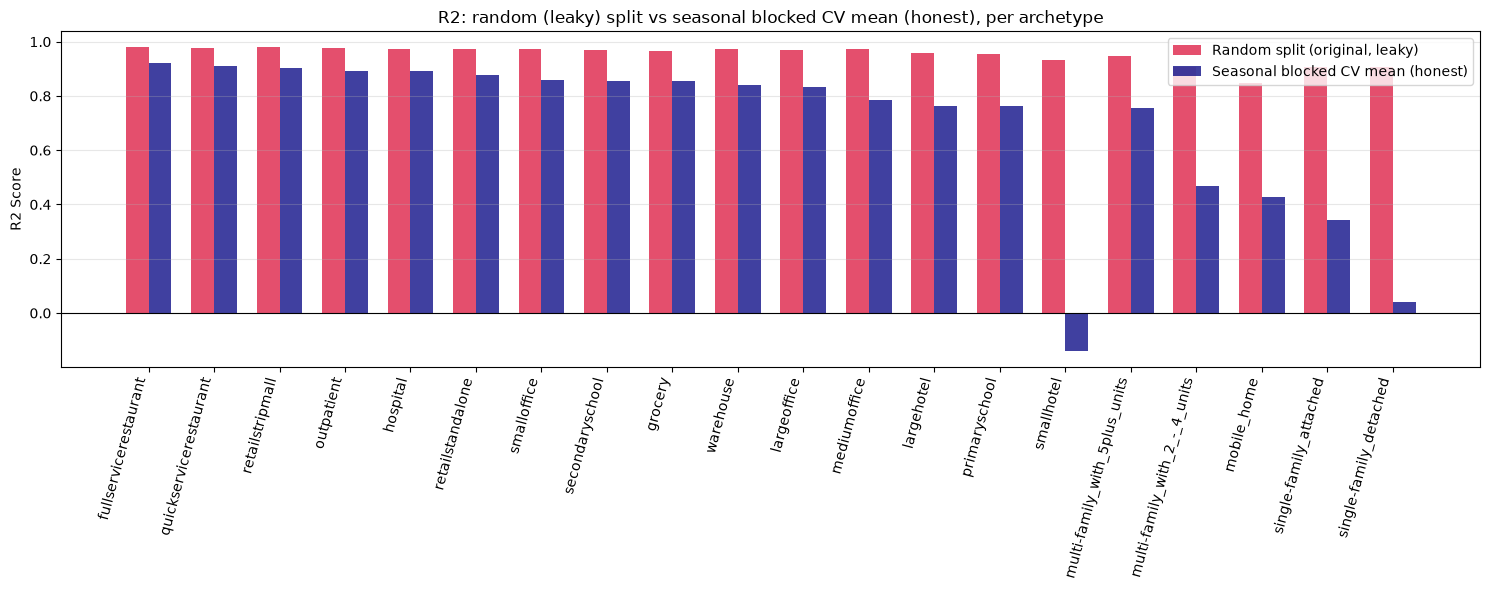
\includegraphics[width=0.95\textwidth]{figures/temporal_train_test_fig1.png}
\caption{R\textsuperscript{2} per archetype: original random split (leaky) versus
seasonal blocked CV mean (honest), still using the (subsequently found to be
incorrect) original weather station.}
\end{figure}

\section{Weather Station Geography Correction}
\label{sec:weather}

\subsection{Bug Discovery}

While investigating the residential weakness identified in Section~\ref{sec:temporal},
the single weather station used throughout the pipeline (station ID
\texttt{G4804610}) was found not to belong to the Coast zone at all. NREL indexes its
weather files by \emph{county}, not by PUMA code, but the original notebooks build
weather station IDs from PUMA codes. Of roughly 50 constructed IDs, only two ever
resolved on NREL's S3 bucket --- by pure numeric coincidence with two unrelated
counties' FIPS codes. Decoded via the official Census county reference,
\texttt{G4804610} corresponds to \textbf{Upton County}, in the Permian Basin of West
Texas, approximately 800\,km from Houston, and \texttt{G4804630} to \textbf{Uvalde
County} in South Texas. Neither is one of the twelve real Coast-zone counties.

This was confirmed directly in the weather data: Upton County averages 50.6\%
relative humidity and spans $-11.7$ to $42.2\,^{\circ}$C, versus Harris County
(Houston)'s 76.4\% average relative humidity and $-7.2$ to $37.8\,^{\circ}$C range --- a
meaningfully drier, more continental climate than the humid Gulf Coast the pipeline is
meant to represent. Every model in the pipeline had been trained and driven by the
wrong region's weather.

\subsection{Fix}

NREL does provide a correct weather file for every Texas county. A
population-weighted blend across the twelve real Coast-zone counties was built,
weighted by residential housing units (already-cached Census B25024 data, no new API
calls needed):

\begin{table}[H]
\centering
\begin{tabular}{lclc}
\toprule
County & Weight & County & Weight \\
\midrule
Harris & 66.84\% & Victoria & 1.40\% \\
Fort Bend & 9.51\% & Matagorda & 0.74\% \\
Montgomery & 8.20\% & Wharton & 0.67\% \\
Galveston & 5.54\% & Waller & 0.64\% \\
Brazoria & 5.15\% & Chambers & 0.60\% \\
 & & Calhoun & 0.45\% \\
 & & Jackson & 0.25\% \\
\bottomrule
\end{tabular}
\caption{Population (housing-unit) weights for the corrected Coast-zone weather
blend.}
\end{table}

All 20 archetype models were retrained through the identical honest (seasonal
blocked CV, full-year final training) protocol from Section~\ref{sec:temporal}.

\subsection{Results}

\begin{figure}[H]
\centering
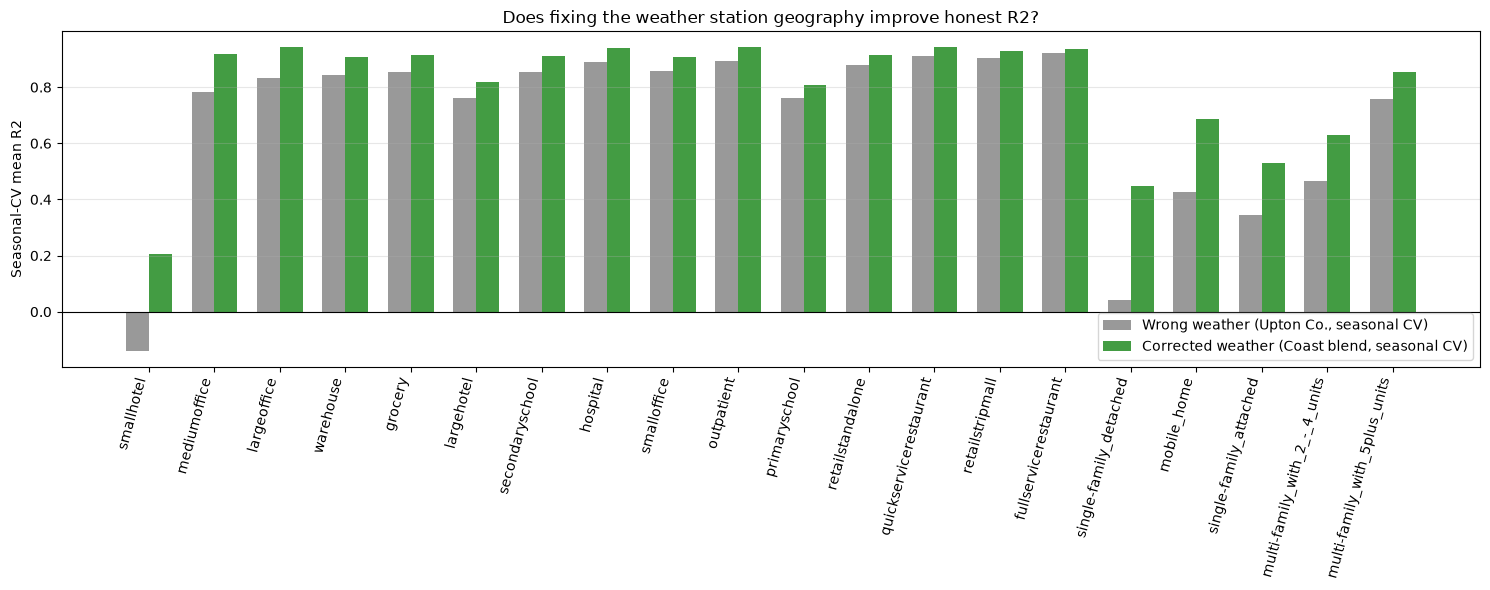
\includegraphics[width=0.95\textwidth]{figures/weather_correction_fig1.png}
\caption{Seasonal-CV mean R\textsuperscript{2} per archetype: wrong weather (Upton
County) vs. corrected weather (Coast-zone population-weighted blend).}
\end{figure}

\begin{table}[H]
\centering
\begin{tabular}{lcc}
\toprule
 & Residential & Commercial \\
\midrule
Wrong weather (honest split) & 0.41 & 0.79 \\
Corrected weather (honest split) & \textbf{0.63} & \textbf{0.86} \\
\bottomrule
\end{tabular}
\caption{Mean seasonal-CV R\textsuperscript{2}, wrong vs. corrected weather.}
\end{table}

The residential gain ($+0.22$) is large, confirming that a substantial part of the
earlier winter/spring weakness was a geography artifact. The system-level Pearson
correlation against ERCOT Coast improved again: \textbf{0.8907 $\rightarrow$
0.8986}, with a reported peak of 26{,}115\,MW.

\subsection{A Related Finding: the True Coast-Zone Footprint}

Cross-referencing the original 56-PUMA Coast zone selection against the official
Census 2010 Tract-to-PUMA relationship file shows that the full PUMA-based zone
definition actually spans \textbf{21 counties}, while the bus-assignment file
(\texttt{tract\_to\_bus\_mapping.csv}) used both for building counts and for the
weather correction above only covers \textbf{12} of those 21. The nine missing
counties (Austin, Colorado, DeWitt, Goliad, Gonzales, Karnes, Lavaca, Liberty,
Wilson) are peripheral, inland counties without any bus of the 200-bus grid nearby.
The 12-county housing-unit total (2{,}645{,}171) matches the paper's already-validated
population figure (2{,}641{,}624 housing units) closely, confirming the 12-county set
is the correct, intentional footprint of the actual synthetic grid --- not an error in
the weather correction, but worth stating explicitly in the paper that the model's
``Coast zone'' does not claim to cover ERCOT's full official Coast weather-zone
boundary, only the actual footprint of the 200-bus grid.

\section{Model Comparison: RandomForest vs. XGBoost vs. LightGBM (Point 6)}
\label{sec:models}

\subsection{Setup}

All three models were run through the identical seasonal blocked 4-fold CV protocol,
on the corrected Coast-zone weather, with reasonable out-of-the-box hyperparameters
(no tuning search) --- a fair baseline-vs-baseline comparison, not a claim of
best-possible performance for any model.

\subsection{Per-Archetype Accuracy and Training Time}

\begin{figure}[H]
\centering
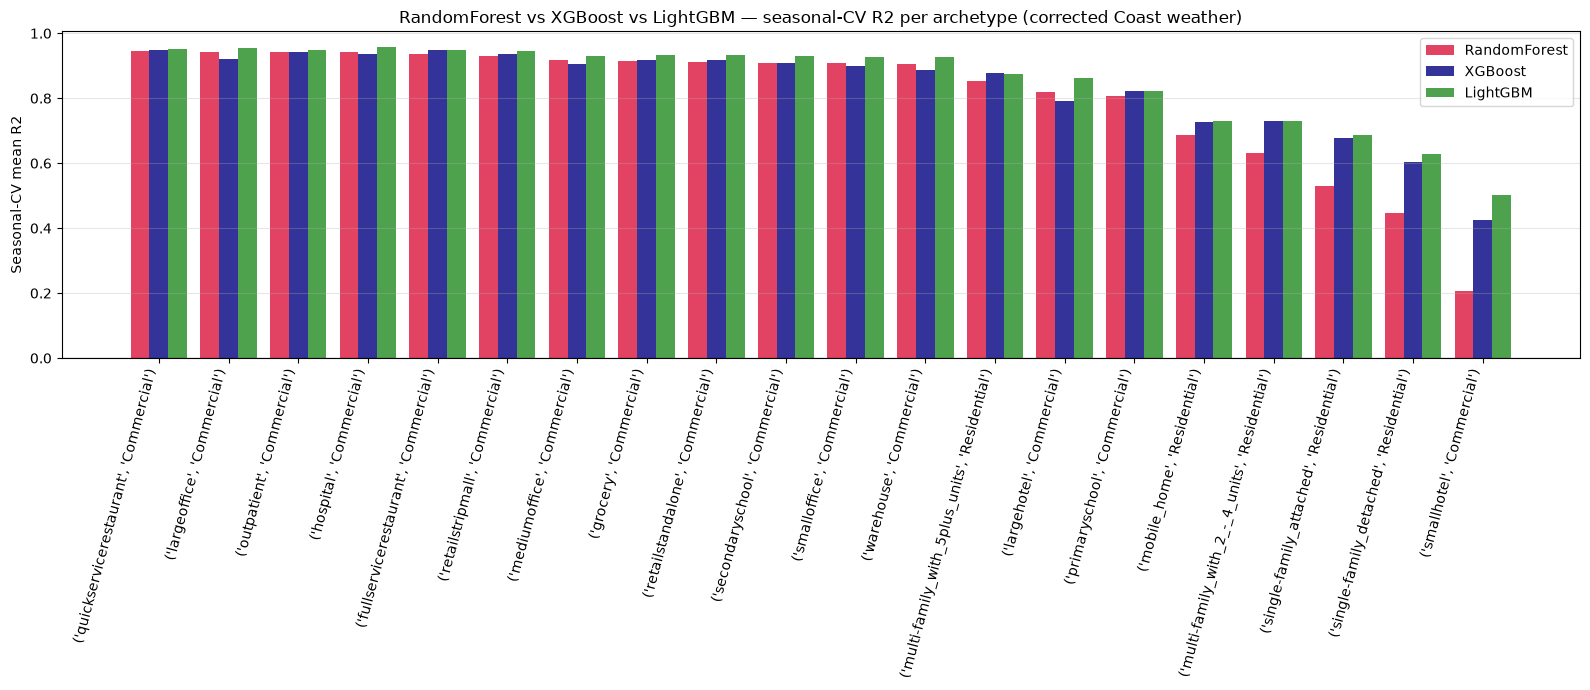
\includegraphics[width=0.95\textwidth]{figures/model_comparison_fig1.png}
\caption{Seasonal-CV R\textsuperscript{2} per archetype: RandomForest vs. XGBoost vs.
LightGBM (corrected Coast weather).}
\end{figure}

\begin{table}[H]
\centering
\begin{tabular}{lccc}
\toprule
 & Residential R\textsuperscript{2} & Commercial R\textsuperscript{2} & Mean fit time (s) \\
\midrule
RandomForest & 0.629 & 0.863 & 0.329 \\
XGBoost & 0.724 & 0.874 & \textbf{0.088} \\
LightGBM & \textbf{0.730} & \textbf{0.899} & 0.372 \\
\bottomrule
\end{tabular}
\caption{Mean seasonal-CV R\textsuperscript{2} and mean per-archetype/fold fit time,
by model.}
\end{table}

LightGBM wins on accuracy in both sectors; XGBoost trains roughly 4$\times$ faster
than the other two. The residential gain from switching model alone
($0.629\rightarrow0.730$) is comparable in magnitude to the earlier weather-station
fix's gain --- a second, independent lever on the residential weakness.

\begin{figure}[H]
\centering
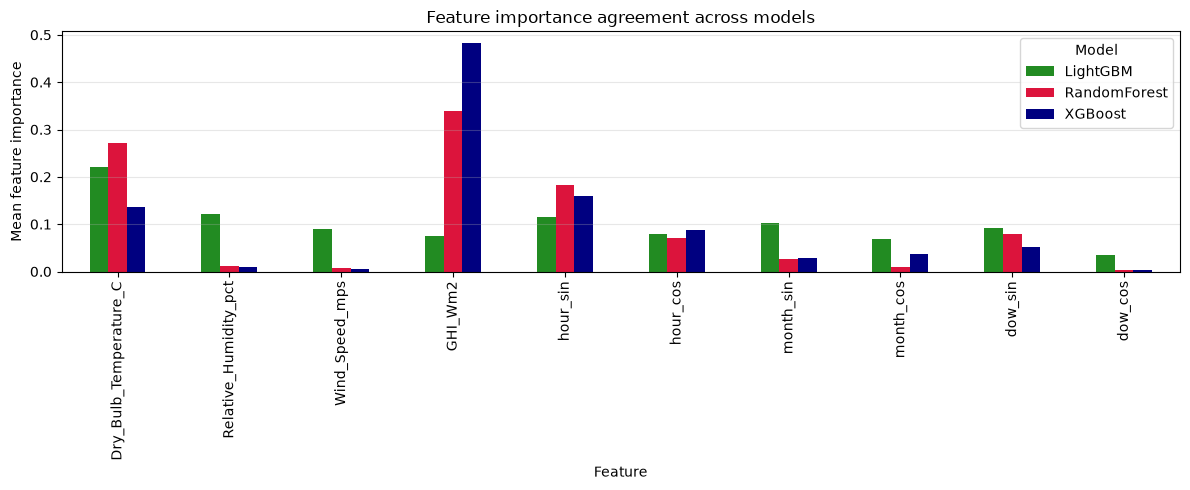
\includegraphics[width=0.8\textwidth]{figures/model_comparison_fig2.png}
\caption{Mean feature importance (normalized to sum to 1 per model) across all 20
archetypes: RandomForest vs. XGBoost vs. LightGBM.}
\end{figure}

\subsection{System-Level Check}

Final full-year production models were trained for all three algorithms, bus-level
profiles regenerated, and the ERCOT Coast Pearson correlation re-checked --- the same
``does it survive aggregation'' test applied to the weather fix.

\begin{figure}[H]
\centering
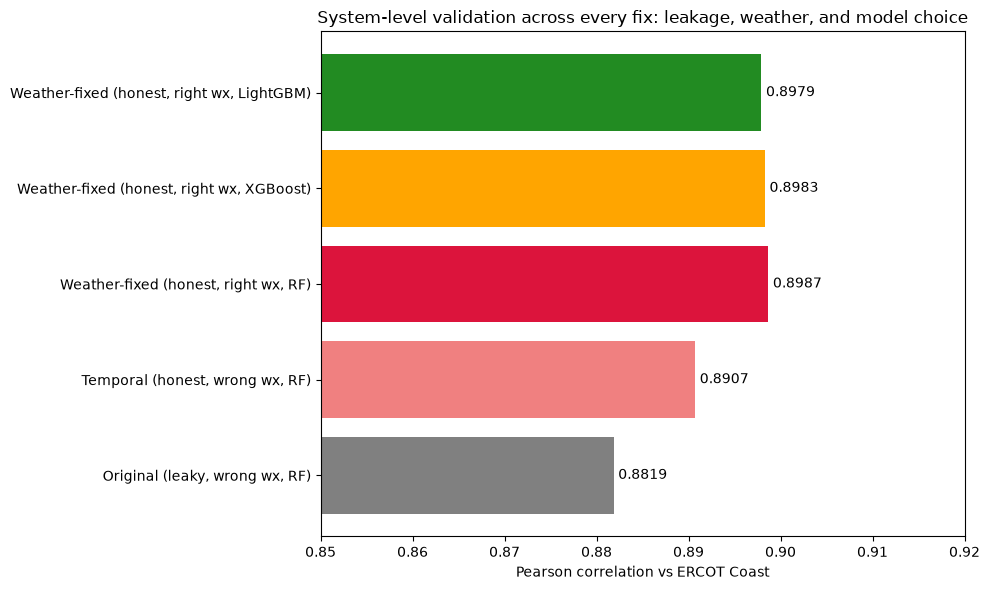
\includegraphics[width=0.85\textwidth]{figures/model_comparison_fig3.png}
\caption{System-level Pearson correlation against ERCOT Coast, across every fix
applied so far (leakage, weather geography, model choice).}
\end{figure}

Despite LightGBM's substantially better per-archetype R\textsuperscript{2}, all three
models land within 0.0008 of each other at the system level (RF 0.8986, XGBoost
0.8983, LightGBM 0.8979) --- statistically indistinguishable. \textbf{Model choice
affects per-building precision, not the aggregate system-level validation number.}
This aggregation-washes-out-precision pattern mirrors the finding for temporal
leakage in Section~\ref{sec:temporal}.

This result supports two equally defensible framings for the paper: (i) retain
RandomForest, since model choice does not affect the headline validation and RF is
the simpler, more interpretable choice, or (ii) adopt LightGBM, since it provides a
materially better per-archetype fit at zero system-level cost. Both are stated here;
the final choice of framing is left open (Section~\ref{sec:nextsteps}).

\subsection{Why No LSTM Was Implemented in Code}

A recurrent/sequence model such as an LSTM learns from a window of past timesteps,
which would mainly help if the target depends on its own recent history beyond what
the instantaneous input features encode --- for example, thermal inertia in a building
(a preceding heat wave keeping indoor temperature elevated after outdoor temperature
drops). This is a plausible mechanism, not implemented in code this round because
(i) it requires a different data representation (contiguous sequence windows, which
interacts awkwardly with the blocked seasonal CV), (ii) it requires a new, heavy
dependency (PyTorch) and materially longer training across 20 archetypes and 4 folds,
and (iii) a cheaper, incremental test of the same hypothesis is available: adding lag
and rolling-window weather features to the existing tabular models. That cheaper test
was run next, in Section~\ref{sec:features}, and confirms the hypothesis.

\section{Feature Engineering}
\label{sec:features}

\subsection{Ablation Design}

Using LightGBM (the Section~\ref{sec:models} winner) held fixed, feature groups were
added incrementally to isolate which additions actually help, under the same seasonal
blocked CV:

\begin{itemize}
    \item \textbf{A (baseline)}: temperature, relative humidity, wind speed, GHI +
    cyclical hour/month/day-of-week (10 features).
    \item \textbf{B = A + free unused weather columns}: wind direction (cyclically
    encoded), direct normal radiation (DNI), diffuse horizontal radiation (DHI) ---
    already present in the cached weather files, unused until now.
    \item \textbf{C = B + degree-hours}: heating and cooling degree-hours at an
    $18\,^{\circ}$C balance point --- the traditional load-forecasting feature.
    \item \textbf{D = C + lag/rolling temperature}: temperature 1\,h and 3\,h prior,
    and a 24\,h rolling mean --- a direct, cheap test of the thermal-inertia hypothesis
    from Section~\ref{sec:models}.
    \item \textbf{E = D + US federal holiday indicator (2018)}.
\end{itemize}

\subsection{Results}

\begin{figure}[H]
\centering
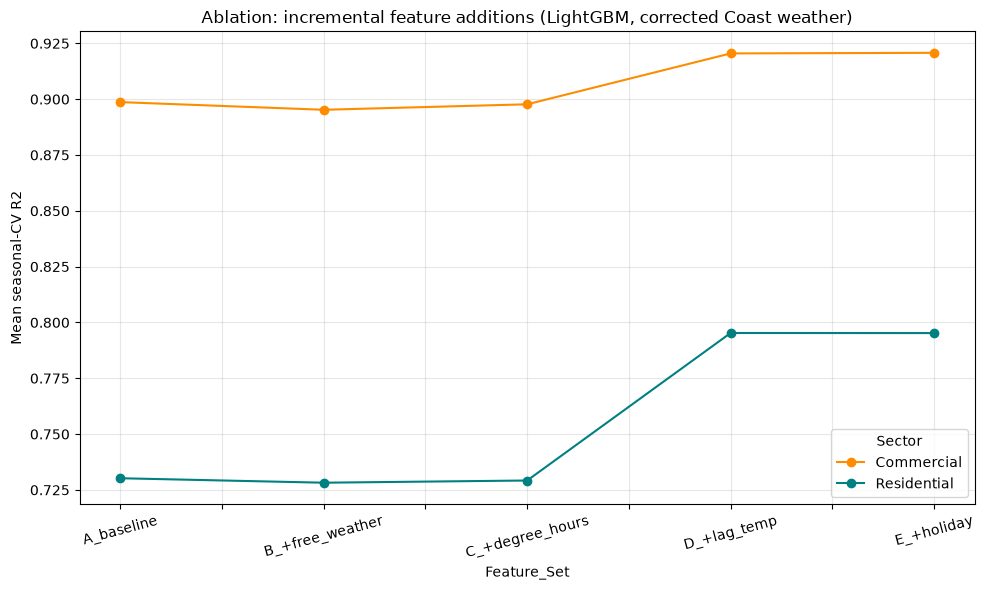
\includegraphics[width=0.85\textwidth]{figures/feature_engineering_fig1.png}
\caption{Ablation: mean seasonal-CV R\textsuperscript{2} by sector, incremental
feature additions (LightGBM, corrected Coast weather).}
\end{figure}

\begin{table}[H]
\centering
\begin{tabular}{lcc}
\toprule
Feature set & Residential R\textsuperscript{2} & Commercial R\textsuperscript{2} \\
\midrule
A: baseline & 0.730 & 0.899 \\
B: + free weather columns & 0.728 & 0.895 \\
C: + degree-hours & 0.729 & 0.898 \\
D: + lag/rolling temperature & \textbf{0.795} & \textbf{0.921} \\
E: + holiday indicator & 0.795 & 0.921 \\
\bottomrule
\end{tabular}
\caption{Mean seasonal-CV R\textsuperscript{2} by sector, per feature set.}
\end{table}

The free unused weather columns and degree-hours contribute essentially nothing.
Lagged/rolling temperature produces the single largest gain seen in any experiment in
this report (residential $0.730\rightarrow0.795$), confirming the thermal-inertia
hypothesis directly and cheaply, without a new model family or dependency. The
holiday indicator adds nothing further on top.

\subsection{System-Level Check}

Final full-year LightGBM models were trained with feature set E, bus-level profiles
regenerated, and the ERCOT correlation re-checked:

\begin{table}[H]
\centering
\begin{tabular}{lcc}
\toprule
 & Pearson vs. ERCOT Coast & Peak (MW) \\
\midrule
LightGBM, baseline features (A) & 0.8979 & 25{,}735 \\
LightGBM, feature set E & \textbf{0.9022} & 25{,}578 \\
\bottomrule
\end{tabular}
\caption{System-level validation, baseline vs. feature-engineered LightGBM.}
\end{table}

Unlike the model-choice comparison in Section~\ref{sec:models}, this change
\emph{does} move the system-level number ($+0.0043$) --- evidence that the
lag/thermal-inertia signal is a genuine physical effect that partially survives
aggregation, not merely per-archetype noise reduction.

\section{Validation Metrics Beyond Aggregate Correlation (Point 5): Full Comparison}
\label{sec:validation}

Point 5 of the review flagged the existing validation as too system-level. This
section revisits every metric proposed there --- coincidence/diversity factor, load
duration curve, diurnal shape, seasonal bias, and a spatial-consistency proxy --- but
now computed across \textbf{all six pipeline versions} produced in this report:
Original, Temporal, Weather-fixed, XGBoost, LightGBM, and Feature-engineered. All six
use the same, not-yet-re-optimized calibration
(\texttt{RES\_SCALE}\,=\,1.9, \texttt{COM\_SCALE}\,=\,1.3, \texttt{IND\_BASE}\,=\,4500\,MW
--- see Section~\ref{sec:nextsteps}). Figures are limited to ERCOT actual + Original +
Weather-fixed + Feature-engineered for legibility, since Section~\ref{sec:models}
already established that model choice alone does not visibly change the aggregate
shape; full numeric tables include all six versions.

\textbf{This section's headline finding is that the story is not uniformly
monotonic.} The Pearson correlation improves with every fix, but several secondary
metrics do not --- a more nuanced and more defensible picture than ``every fix improved
everything.''

\subsection{Pearson Correlation, Peak, and Load Factor}

\begin{table}[H]
\centering
\begin{tabular}{lccc}
\toprule
Pipeline & Pearson vs. ERCOT & Peak (MW) & Load Factor \\
\midrule
Original & 0.8818 & 24{,}418 & 0.582 \\
Temporal & 0.8907 & 24{,}604 & 0.578 \\
Weather-fixed & 0.8986 & 26{,}115 & 0.544 \\
XGBoost & 0.8983 & 26{,}279 & 0.541 \\
LightGBM & 0.8979 & 25{,}735 & 0.552 \\
Feature-engineered & \textbf{0.9022} & 25{,}578 & 0.556 \\
\midrule
ERCOT Actual & --- & 20{,}270 & 0.600 \\
\bottomrule
\end{tabular}
\caption{Pearson correlation, peak, and load factor across all six pipeline
versions.}
\end{table}

Pearson correlation improves essentially monotonically. Load factor does
\textbf{not}: Original (0.582) is actually the closest of all six to ERCOT's 0.600,
and the weather fix moves it further away (0.544) before feature engineering
partially recovers it (0.556). The corrections that improved hour-by-hour
correlation made the estimated stack slightly peakier relative to ERCOT actual than
the uncorrected pipeline was.

\subsection{Coincidence and Diversity Factor}

\begin{table}[H]
\centering
\small
\begin{tabular}{lccc}
\toprule
Pipeline & CF, Residential & CF, Commercial & CF, Combined \\
\midrule
Original & 0.9983 & 0.9984 & 0.9625 \\
Temporal & 0.9957 & 0.9967 & 0.9789 \\
Weather-fixed & 0.9996 & 0.9961 & 0.9857 \\
XGBoost & 1.0000 & 0.9985 & 0.9896 \\
LightGBM & 0.9997 & 0.9981 & 0.9885 \\
Feature-engineered & 1.0000 & 0.9985 & 0.9843 \\
\bottomrule
\end{tabular}
\caption{Coincidence factor, residential-only, commercial-only, and combined bus
sets, all six versions.}
\end{table}

Within-sector CF stays pinned near 1.0 across every version --- a structural property
of the current single, zone-wide weather series design (Section~\ref{sec:nextsteps}),
unaffected by any split, weather, model, or feature fix tried so far. The
\emph{combined} (residential + commercial) CF trends from 0.963 toward 0.99 as fixes
are applied, meaning \emph{less} diversity between residential and commercial peak
timing, not more --- plausibly because better models converge more tightly on the same
dominant driver (temperature), so the two sectors' peaks align more closely.

\subsection{Load Duration Curve}

\begin{figure}[H]
\centering
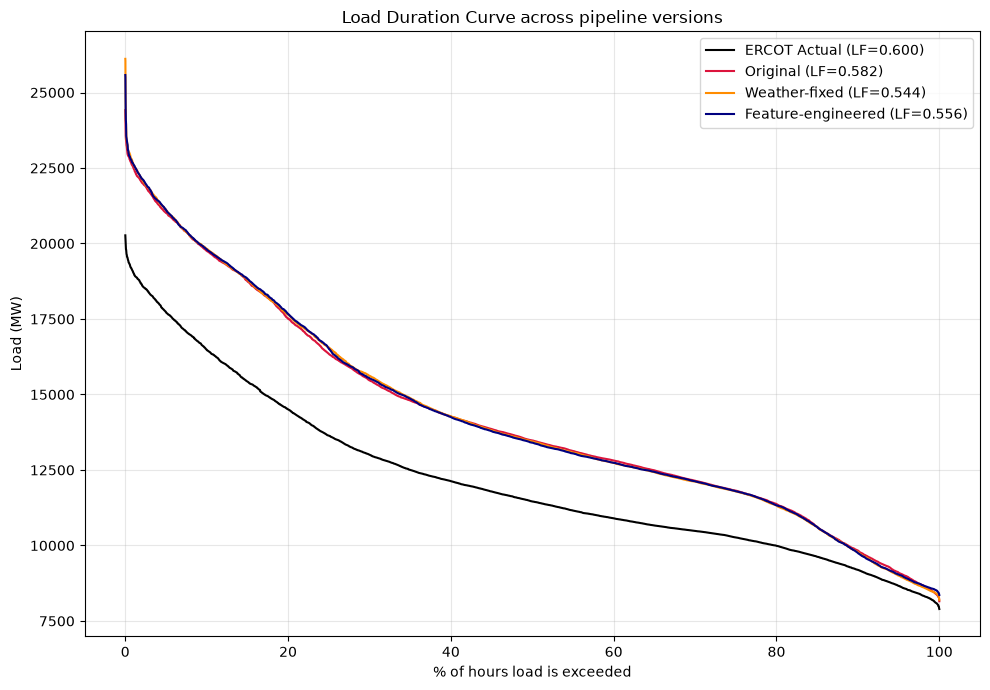
\includegraphics[width=0.8\textwidth]{figures/validation_full_fig1.png}
\caption{Load duration curve across pipeline versions. The systematic vertical gap
between every estimated curve and ERCOT actual reflects the not-yet-re-optimized
calibration scale factors, not a shape mismatch.}
\end{figure}

\subsection{Diurnal Shape}

\begin{figure}[H]
\centering
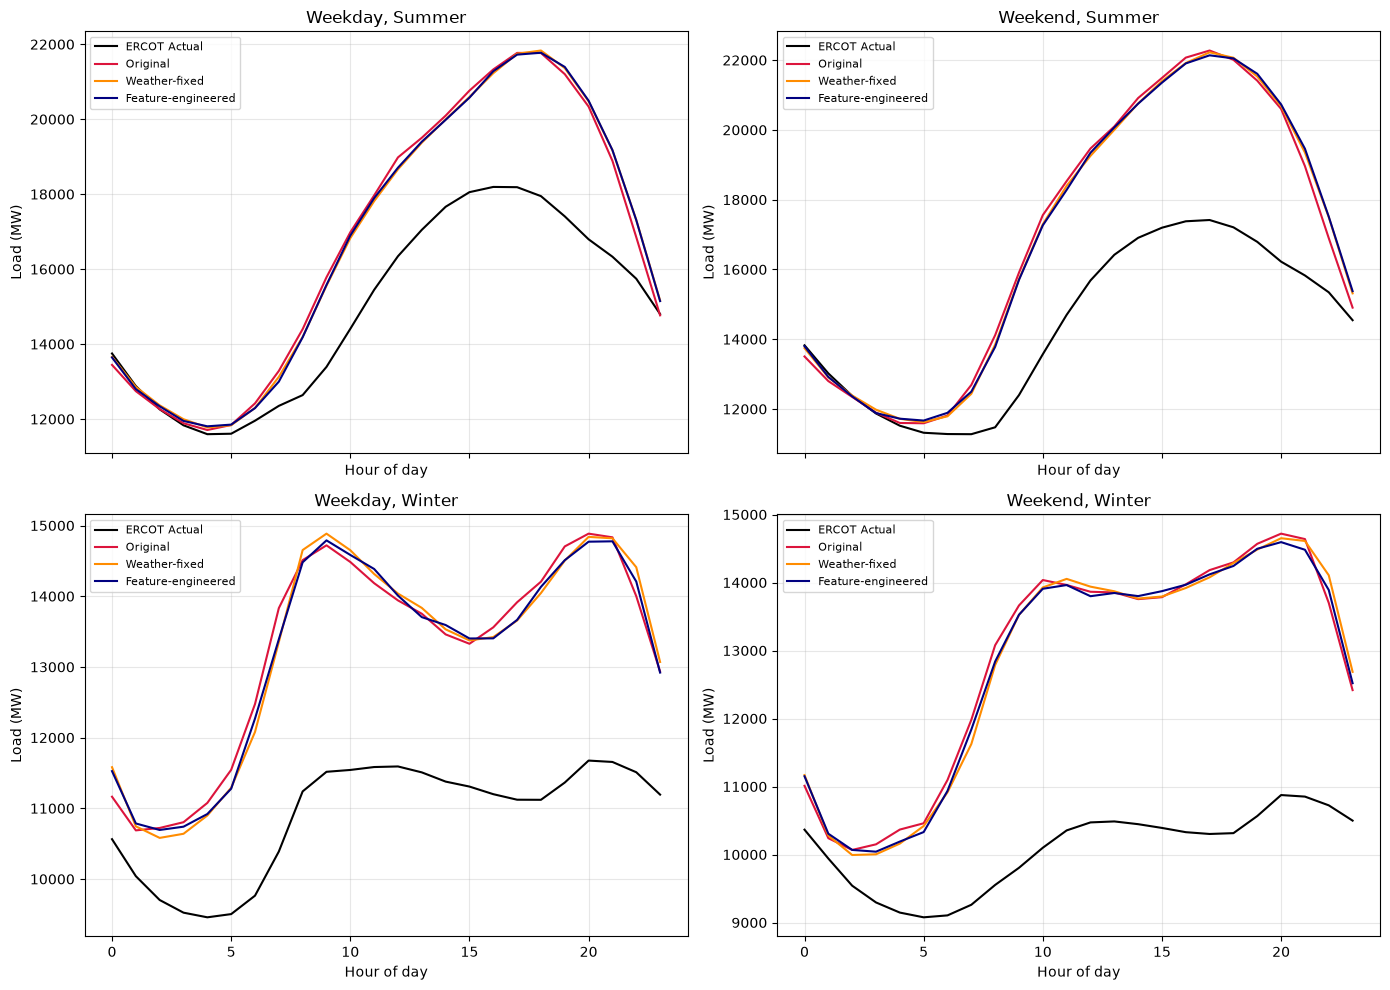
\includegraphics[width=0.95\textwidth]{figures/validation_full_fig2.png}
\caption{Average diurnal load shape by weekday/weekend $\times$ summer/winter, ERCOT
actual vs. Original vs. Weather-fixed vs. Feature-engineered.}
\end{figure}

\begin{table}[H]
\centering
\small
\begin{tabular}{lcccc}
\toprule
Pipeline & Wd. Summer & We. Summer & Wd. Winter & We. Winter \\
\midrule
Original & 0.9757 & 0.9483 & 0.8739 & 0.7668 \\
Temporal & 0.9808 & 0.9610 & 0.9192 & 0.8047 \\
Weather-fixed & 0.9807 & 0.9600 & \textbf{0.9223} & \textbf{0.8116} \\
XGBoost & 0.9809 & 0.9600 & 0.9173 & 0.8090 \\
LightGBM & 0.9808 & 0.9614 & 0.9192 & 0.7997 \\
Feature-engineered & 0.9801 & 0.9610 & 0.9151 & 0.7978 \\
\bottomrule
\end{tabular}
\caption{Correlation of average diurnal shape (not level) against ERCOT actual, all
six versions.}
\end{table}

The winter-weekend condition --- the single weakest metric identified anywhere in this
report --- improves substantially from Original (0.767) to a peak at Weather-fixed
(0.812), but then \textbf{drifts back down} through XGBoost, LightGBM, and
Feature-engineered (0.798), still comfortably above the original value but below the
weather-fix peak. The temporal and weather-geography fixes are what actually repaired
this particular metric; the later model-choice and feature-engineering refinements
improved per-archetype accuracy and the overall Pearson correlation without further
improving this specific shape sub-metric --- in fact trading a small amount of it away.

\subsection{Seasonal Monthly Bias}

\begin{figure}[H]
\centering
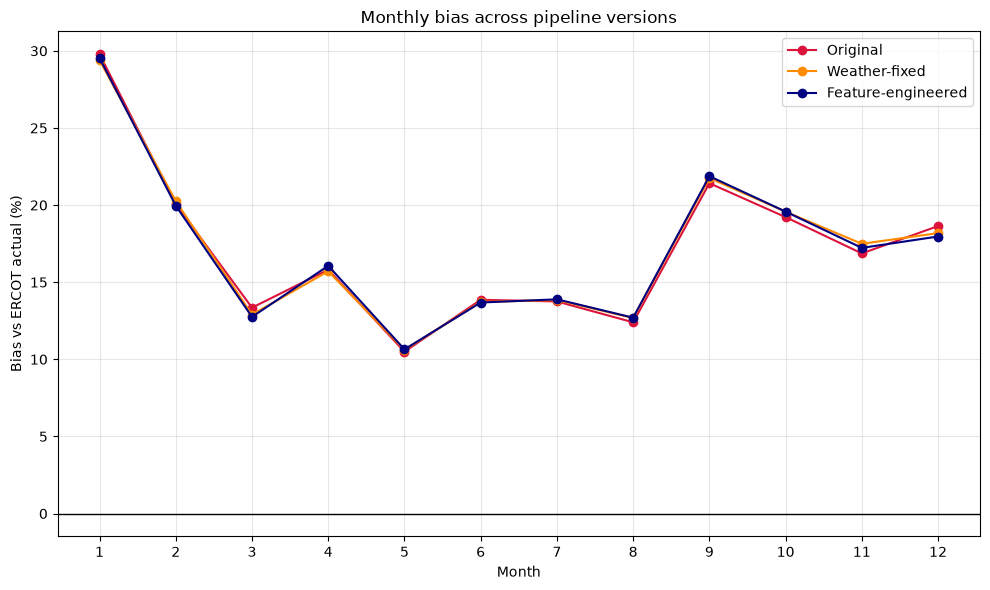
\includegraphics[width=0.8\textwidth]{figures/validation_full_fig3.png}
\caption{Monthly bias (\%) vs. ERCOT actual, across pipeline versions.}
\end{figure}

Bias is positive in every month for every version (range: $+10.5\%$ in May to
$+29.8\%$ in January), and the three plotted versions track each other closely ---
differences between versions are mostly under one percentage point per month. This
is consistent with a calibration-scale issue rather than a shape issue: the pipeline
over-predicts uniformly across the year, which the RES\_SCALE/COM\_SCALE
recalibration (Section~\ref{sec:nextsteps}) is expected to address directly.

\subsection{Spatial Consistency Proxy}

Correlation between per-bus annual energy and per-bus building/sqft count is
\textbf{effectively invariant} across all six pipeline versions: residential is
identical to four decimal places (0.9479), commercial varies by one unit in the
fourth decimal (0.8917--0.8918). This confirms the proxy is
insensitive to every fix and refinement tried --- expected, since building counts and
the sqft mapping are unchanged Census/ArcGIS inputs across all six versions, and this
metric was always primarily a plumbing sanity check rather than an independent
spatial validation.

\subsection{Out of Scope: Comparison Against Prior Synthetic-Grid Methods}

Review point 9 requested a quantitative comparison against a prior proportional
load allocation method (referenced as ``Hanyue's method''). This has not been
implemented --- the exact method description is not yet available and is needed before
this comparison can be built.

\subsection{Section Takeaway}

The temporal-leakage and weather-geography fixes (Sections~\ref{sec:temporal}
and~\ref{sec:weather}) are the corrections that improved the secondary shape metrics
(load duration curve shape, winter-weekend diurnal match) as well as the headline
correlation. The later model-choice and feature-engineering refinements
(Sections~\ref{sec:models} and~\ref{sec:features}) mainly improved per-archetype
accuracy and the aggregate Pearson number, while leaving flat --- or in one case
(winter-weekend diurnal shape) slightly trading off --- some of these secondary
metrics. Reporting this honestly, rather than claiming uniform improvement, is a
stronger and more defensible position for reviewers.

\section{Combined Progression of Results}

\begin{table}[H]
\centering
\small
\begin{tabular}{lcccc}
\toprule
Pipeline version & Res.\ R\textsuperscript{2} & Com.\ R\textsuperscript{2} & Pearson & Peak (MW) \\
\midrule
Original (leaky split, wrong weather, RF) & 0.90$^{*}$ & 0.97$^{*}$ & 0.8818 & 24{,}418 \\
+ honest temporal split & 0.41 & 0.79 & 0.8907 & 24{,}604 \\
+ corrected weather geography & 0.63 & 0.86 & 0.8986 & 26{,}115 \\
+ LightGBM (vs.\ RandomForest) & 0.73 & 0.90 & 0.8979 & 25{,}735 \\
+ feature engineering (lag temperature) & \textbf{0.80} & \textbf{0.92} & \textbf{0.9022} & 25{,}578 \\
\bottomrule
\end{tabular}
\caption{Full progression across every correction applied. Pearson is measured against
ERCOT Coast actual load, whose 2018 peak is 20{,}270\,MW. $^{*}$leakage-inflated,
not comparable to the honest values below them.}
\label{tab:progression}
\end{table}

Two independent bugs (temporal leakage, weather geography) and two optional
improvements (model choice, feature engineering) were tested under one consistent,
non-leaking evaluation protocol throughout. The Pearson correlation against ERCOT
Coast actual load improved overall from 0.8818 to 0.9022 across the full sequence of
changes --- though not strictly monotonically: the model-choice step dips slightly
(0.8986 $\rightarrow$ 0.8979) before feature engineering recovers and exceeds it. The
per-archetype R\textsuperscript{2} figures reported are
now honest, non-inflated estimates rather than the originally-reported,
leakage-inflated values. As detailed in Section~\ref{sec:validation}, even this
overall improvement holds for the headline correlation specifically, not for every
secondary validation metric.

\section{Statewide Extension to All Five Texas IECC Climate Zones}
\label{sec:statewide}

The previous sections all concern the single, original 200-bus Coast case study (IECC
zone 2A). Section~\ref{sec:nextsteps} of the prior phase of this work listed
``extension to all of Texas'' as blocked, specifically on a missing bus-to-load spatial
mapping (substation locations/topology) for any region beyond the existing 200-bus
Coast grid. Two new GIS join files have since been obtained, built for a genuinely
new, denser statewide synthetic grid: \texttt{tract\_to\_bus\_mapping\_statewide\_%
ExportTable.csv} (6{,}896 census tracts $\rightarrow$ 3{,}426 buses, residential) and
\texttt{zcta\_bus\_mapping\_tx\_final.csv} (2{,}031 ZCTAs $\rightarrow$ bus, commercial).
This is \emph{not} an extension of the original 200-bus Coast grid: a 1\,km
nearest-substation match against the old Coast file only recovers 72 of the 200 old
buses, confirming it is a different, denser grid built independently.

\subsection{Zone Definitions and New Bus Grid}

An authoritative county $\rightarrow$ IECC climate-zone crosswalk was built from NREL's
own \texttt{spatial\_tract\_lookup\_table.csv} (the same geographic reference ResStock
itself ships with), rather than a third-party map --- deliberately avoiding the exact
kind of geography mismatch that caused the original PUMA-vs-county weather bug
(Section~\ref{sec:weather}). No Texas county is split across two IECC zones.

\begin{table}[H]
\centering
\small
\begin{tabular}{lccl}
\toprule
Zone & Counties & Buses & Description \\
\midrule
2A & 79 & 1{,}883 & Very Hot-Humid (includes the original 12-county Coast footprint) \\
2B & 14 & 81 & Hot-Dry \\
3A & 63 & 1{,}219 & Warm-Humid (DFW / North / East Texas) \\
3B & 70 & 194 & Warm-Dry (West Texas / Permian Basin) \\
4B & 28 & 52 & Mixed-Dry (Texas Panhandle / Far West) \\
\bottomrule
\end{tabular}
\caption{The five Texas IECC climate zones covering all 254 counties. The bus counts
are those of the initial nearest-bus mapping; the authoritative bus table adopted in
Section~\ref{sec:areasplit} covers the full grid of 6{,}717 buses (2A 3{,}580, 2B 246,
3A 2{,}142, 3B 625, 4B 124), with identical county assignments.}
\label{tab:zones}
\end{table}

\subsection{Two New Geography Issues Found}

\textbf{Census tract vintage mismatch.} While building the first zone (2A), 740 of its
1{,}883 buses (39\%) initially came out with zero residential building count. Root
cause: the new statewide bus mapping is built on \emph{2020} Census tract boundaries
(Harris County = 1{,}115 tracts), while the cached Census B25024 file used throughout
Sections~\ref{sec:baseline}--\ref{sec:features} is on \emph{2010} tract boundaries
(Harris County = 786 tracts --- correct for, and only for, the original Coast-only
file). Fixed by re-fetching Census B25024 on the 2022 ACS5 vintage (confirmed to
return exactly 1{,}115 Harris tracts). After the fix, zero-count buses dropped to
under 1\% in every zone. This is the same class of bug as the original weather-station
geography issue (Section~\ref{sec:weather}) --- a silent geography/vintage mismatch ---
caught the same way, by checking a suspicious diagnostic number instead of trusting a
silent join.

\textbf{Structural commercial bus-coverage gap.} Unlike the tract-to-bus join
(6{,}896 tracts for 3{,}426 buses, ratio $>1$, so nearly every bus receives at least
one tract), the ZCTA-to-bus join has only 2{,}031 ZCTAs for 3{,}426 buses (ratio
$<1$). Since each ZCTA is matched to its single nearest bus, at most 2{,}031 buses can
ever receive commercial load this way, and in practice only 1{,}598 (47\%) do ---
compared to 92.5\% coverage on the original, much smaller and denser 200-bus Coast
grid. This is not a code bug but a structural property of the provided file: it
concentrates commercial load onto fewer buses than physically realistic rather than
losing or double-counting it (region-level totals are unaffected, confirmed by the
cross-check in Section~\ref{sec:crosscheck}), but it does mean per-bus commercial
values are not reliable for any downstream use that inspects individual buses (e.g.\
power-flow studies) rather than regional aggregates. \emph{Resolved in
Section~\ref{sec:areasplit}}: an area-split join (100 equal-area parts per ZCTA) raises
coverage of load-carrying buses to 96.1\%, and confirms the claim made here that
region-level totals were unaffected --- every zone-aggregate number in this section is
unchanged by the fix.

\subsection{Methodology}

The already-validated Coast methodology (Sections~\ref{sec:temporal}--%
\ref{sec:features}) is reused as-is, generalized per zone, with no re-derivation of
settled conclusions:

\begin{itemize}
    \item Population-weighted county weather blend (Section~\ref{sec:weather}'s fix),
    generalized from Coast's 12 counties to each zone's full county list.
    \item Cyclical calendar features plus lagged/rolling temperature
    (Section~\ref{sec:features}'s winning feature set).
    \item LightGBM (Section~\ref{sec:models}'s winning model).
    \item Blocked seasonal 4-fold cross-validation for the honest R\textsuperscript{2}
    estimate; full-year training for the deployed model.
    \item Commercial: identical CBP/ZBP employment methodology as the original Coast
    \texttt{commercial.ipynb} (NAICS $\rightarrow$ ComStock-archetype mapping,
    CBECS-derived sqft/employee factors), reusing the already-statewide ZBP raw file
    (all Texas ZIP prefixes) rather than re-downloading it per zone.
\end{itemize}

\subsection{Honest Accuracy Results}

\begin{figure}[H]
\centering
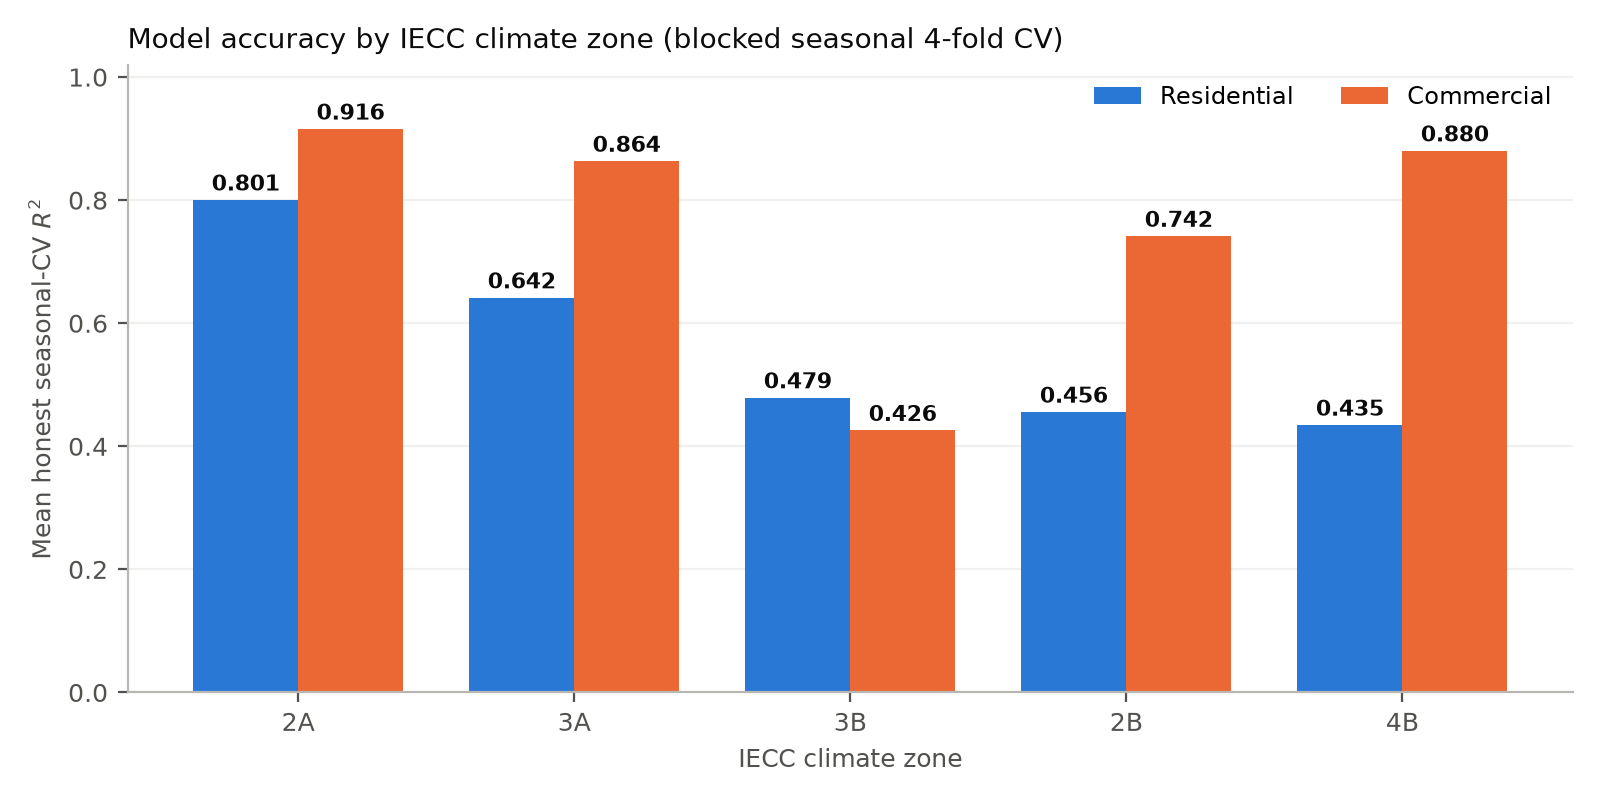
\includegraphics[width=0.75\textwidth]{figures/statewide_r2_by_zone_fig1.png}
\caption{Mean honest seasonal-CV R\textsuperscript{2} by IECC zone, residential vs.
commercial.}
\label{fig:statewide_r2}
\end{figure}

\begin{table}[H]
\centering
\small
\begin{tabular}{lcc}
\toprule
Zone & Residential mean R\textsuperscript{2} & Commercial mean R\textsuperscript{2} \\
\midrule
2A & 0.801 & 0.916 \\
3A & 0.642 & 0.864 \\
3B & 0.479 & 0.426 \\
2B & 0.456 & 0.742 \\
4B & 0.435 & 0.880 \\
\bottomrule
\end{tabular}
\caption{Honest seasonal-CV mean R\textsuperscript{2}, ranked by residential
difficulty. Zone 2A (Coast's own climate) is clearly easiest; drier/more continental
zones are harder, plausibly a mix of a more complex weather-load relationship (real
heating seasons, not purely cooling-dominated) and smaller sample sizes. Values are
from the current run; they shifted by up to 0.014 from the first statewide pass
because the area-split allocation (Section~\ref{sec:areasplit}) slightly changes each
zone's county weather weights. Model choice, features and protocol are unchanged.}
\label{tab:statewide_r2}
\end{table}

Commercial accuracy is generally higher than residential per zone, \emph{except} in
3B, where it collapses to 0.426. Four zone/archetype combinations have a genuinely
negative mean R\textsuperscript{2}: 3B \texttt{largehotel} ($-1.36$, as low as $-3.14$
in its worst season), 3B \texttt{smallhotel} ($-0.28$), 2B \texttt{smallhotel}
($-0.26$), and 3B \texttt{grocery} ($-0.10$). This was checked against a ComStock sample-size artifact
and ruled out: 3B's \texttt{largehotel} archetype has \emph{more} underlying sampled
buildings (\texttt{models\_used}\,=\,881) than 2A's (361). The most likely explanation
is that hotel demand in this region (Permian Basin) is driven by non-weather factors
(oilfield workforce cycles) that a weather-only feature set cannot capture --- a genuine
``no signal'' finding, not an artifact.

\subsection{Cross-Check Against the Already-Validated Coast Pipeline}
\label{sec:crosscheck}

Because the new statewide grid does not share bus IDs with the original 200-bus Coast
grid (Section~\ref{sec:statewide}), a bus-level comparison is not possible. Instead,
the new zone-2A reconstruction is restricted to buses inside the original 12 Coast
counties (1{,}505 matching buses on the full grid) and compared, at the aggregate
level, against the already-validated Coast-only reconstruction
(Section~\ref{sec:features}'s \texttt{\_featureeng} output).

\begin{table}[H]
\centering
\small
\begin{tabular}{llccc}
\toprule
Stack & Version & Peak (MW) & Annual mean (MW) & $r$ \\
\midrule
\multirow{2}{*}{Residential} & New (Coast-county subset, 1{,}505 buses) & 11{,}552.6 & 4{,}895.1 & \multirow{2}{*}{0.9965} \\
 & Old (already-validated Coast pipeline) & 10{,}084.0 & 4{,}260.3 & \\
\midrule
\multirow{2}{*}{Commercial} & New (Coast-county subset, 1{,}505 buses) & 2{,}606.3 & 1{,}291.9 & \multirow{2}{*}{0.9993} \\
 & Old (already-validated Coast pipeline) & 2{,}534.7 & 1{,}245.8 & \\
\bottomrule
\end{tabular}
\caption{Cross-check: the new statewide methodology, restricted to the original 12
Coast counties, reproduces the already-validated Coast-only reconstruction closely on
both stacks --- the shape correlation is what this test is for, and it is essentially
perfect. The level gap is larger on residential (+14.6\%) than commercial (+2.8\%)
because the two footprints are not the same set: the full grid places 1{,}505 buses in
those 12 counties against the old grid's 200, so the subset captures more of the
counties' housing. The zone-wide weather blend (98 counties for the 2A run) diluting
the Coast-specific 12-county blend also contributes.}
\label{tab:crosscheck}
\end{table}

\subsection{Statewide Totals (Uncalibrated)}

\begin{table}[H]
\centering
\small
\begin{tabular}{lcc}
\toprule
Zone & Residential peak (MW) & Commercial peak (MW) \\
\midrule
2A & 25{,}098.4 & 5{,}305.7 \\
3A & 17{,}101.3 & 3{,}343.4 \\
3B & 2{,}518.3 & 595.0 \\
2B & 1{,}020.1 & 294.1 \\
4B & 594.2 & 100.5 \\
\midrule
\textbf{Statewide total (coincident)} & \textbf{43{,}161.1} & \textbf{9{,}434.3} \\
\bottomrule
\end{tabular}
\caption{Per-zone and statewide peak load, residential and commercial, uncalibrated
(no RES\_SCALE/COM\_SCALE applied) and with no industrial component anywhere except
Coast's flat placeholder (not included in this table). The statewide row is the peak
of the summed statewide series, not the sum of the per-zone peaks, which is why it
falls below the column total: the five zones do not peak in the same hour.}
\label{tab:statewide_totals}
\end{table}

\section{Coast Recalibration}
\label{sec:recalibration}

This section resolves the first open item from Section~\ref{sec:nextsteps} of the
previous phase.

\subsection{Bug Discovery}

Two independent problems were found while revisiting the Coast calibration
(\texttt{plot\_all.ipynb}). First, the grid-search cell contained a broken line
(\texttt{results\_matrix\ =\ .astype(float)}, a syntax error with the variable name
missing) that could never have executed as written --- meaning the notebook's stored
outputs (Pearson 0.8806, RES\_SCALE=1.9/COM\_SCALE=1.3) were stale artifacts from some
earlier working state, not reproducible from the code as it sat in the repository.
Second, and more importantly, every cell in this notebook was still reading the
\emph{original}, pre-fix profile files (no suffix), not \texttt{\_featureeng} --- meaning
the ``official'' Coast calibration had never been re-run against any of the three
corrections in Sections~\ref{sec:temporal}--\ref{sec:features}, exactly the
staleness this open item had already flagged.

\subsection{Fix and Results}

The syntax error was fixed, every cell was switched to read \texttt{\_featureeng}, and
the grid search was re-run.

\begin{figure}[H]
\centering
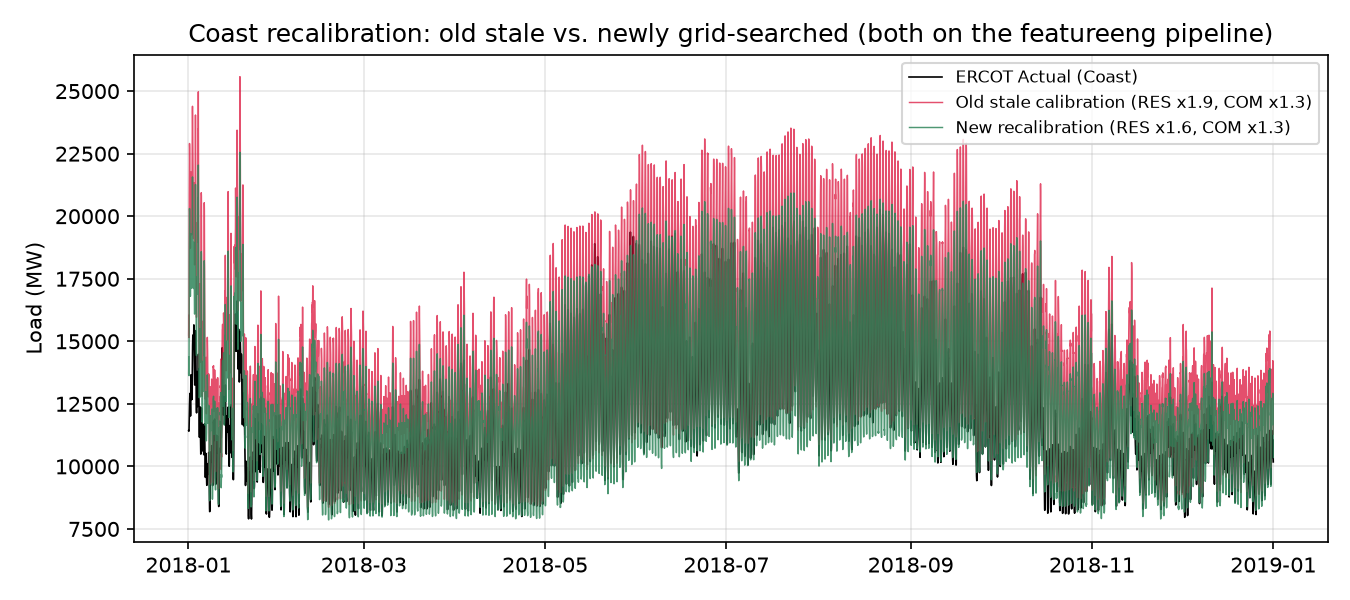
\includegraphics[width=0.85\textwidth]{figures/recalibration_fig1.png}
\caption{Old stale calibration vs.\ newly recalibrated total, both applied to the
current best (\texttt{\_featureeng}) pipeline, vs.\ ERCOT Coast actual.}
\label{fig:recalibration}
\end{figure}

\begin{table}[H]
\centering
\small
\begin{tabular}{lcccc}
\toprule
Calibration & Peak (MW) & Pearson & MAE (MW) & RMSE (MW) \\
\midrule
Old: RES\,1.9 / COM\,1.3 (stale) & 25{,}577.8 & 0.9022 & 2{,}116.7 & 2{,}625.4 \\
\textbf{New: RES\,1.6 / COM\,1.3} & \textbf{22{,}552.6} & \textbf{0.9024} & \textbf{1{,}201.4} & \textbf{1{,}550.9} \\
\bottomrule
\end{tabular}
\caption{ERCOT Coast actual peak: 20{,}269.8\,MW. Pearson correlation is near
scale-invariant and barely moves, but the old calibration was overcorrecting for a
weaker, pre-fix pipeline: the absolute error nearly halves under the new calibration.
\textbf{RES\_SCALE=1.6, COM\_SCALE=1.3 is the number to cite going forward.}}
\label{tab:recalibration}
\end{table}

\section{Validation Beyond Coast: an ERCOT Weather-Zone Crosswalk}
\label{sec:ercot-crosswalk}

\emph{Superseded by Section~\ref{sec:ercot8}, which validates all eight ERCOT weather
zones from a per-bus crosswalk contained in the grid model itself. This section is
retained because its method --- and the Panhandle finding below --- document how the
problem was approached before that field was available, and because its conclusion about
West Texas was correct and is reproduced by the better method.}

Coast is the only IECC zone with a direct, real validation number, because ERCOT
publishes actual historical load by its own eight \emph{weather zones} (\texttt{COAST},
\texttt{EAST}, \texttt{FWEST}, \texttt{NORTH}, \texttt{NCENT}, \texttt{SOUTH},
\texttt{SCENT}, \texttt{WEST}) --- a completely different zoning scheme from NREL's five
IECC \emph{climate} zones used throughout this report. No public, machine-readable
county-to-ERCOT-weather-zone crosswalk exists (confirmed via search: ERCOT publishes
only a picture map, \texttt{ercot.com/news/mediakit/maps}). One was built here by
visually reading that map together with ERCOT's separate county-participation map
(which does precisely show an in-ERCOT/not-in-ERCOT flag per county), anchored on the
known latitude/longitude of the twelve cities labeled on the weather-zone map.

A notable finding while doing this: the Texas Panhandle is \emph{not} uniformly
outside ERCOT, as had been assumed earlier in this project. Roughly half its counties
(including Amarillo/Potter/Randall) show as ``in ERCOT'' on the official
county-participation map, which contradicts the common description of Amarillo as
Southwest Power Pool (SPP) territory. Given this contradiction, IECC zone 4B was left
out of this validation pass entirely rather than risk an overconfident partial claim.
Extending precise ERCOT-zone validation to zones 2A (beyond Coast), 2B, 3A, and 4B
appeared at the time to need real GIS shapefiles for ERCOT's weather zones, not a
hand-read map --- each of those zones straddles multiple ERCOT weather zones along
boundaries that were not reliably resolvable visually. That turned out not to be the
binding constraint: the grid model itself carries the assignment
(Section~\ref{sec:ercot8}).

\subsection{Zone 3B: West Texas / Permian Basin}

Zone 3B was chosen as the one unambiguous case: 67 of its 70 counties map cleanly to
ERCOT's \texttt{WEST} and \texttt{FWEST} zones combined. The three excluded counties
are El Paso and Hudspeth (genuinely outside ERCOT, in the Western Interconnection) and
Hemphill (the one ambiguous Panhandle-adjacent corner). The zone-3B bus-level
reconstruction (residential + commercial, Section~\ref{sec:statewide}) is restricted
to these 67 counties' buses and compared to ERCOT's real \texttt{WEST}+\texttt{FWEST}
total.

\begin{figure}[H]
\centering
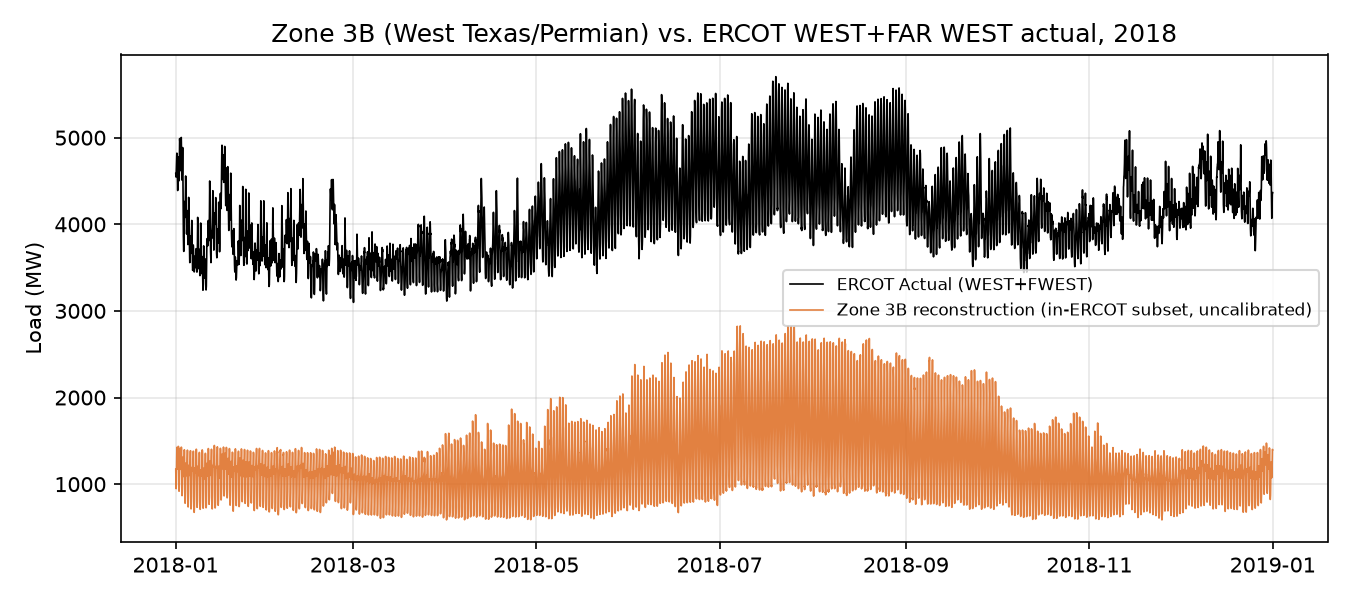
\includegraphics[width=0.85\textwidth]{figures/zone3b_vs_ercot_fig1.png}
\caption{Zone 3B reconstruction (in-ERCOT county subset, uncalibrated) vs.\ ERCOT
WEST+FAR WEST actual load, 2018.}
\label{fig:zone3b}
\end{figure}

\begin{table}[H]
\centering
\small
\begin{tabular}{lc}
\toprule
& Zone 3B (vs.\ ERCOT WEST+FWEST) \\
\midrule
ERCOT actual peak & 5{,}704.2\,MW \\
Reconstruction peak (uncalibrated) & 2{,}827.2\,MW \\
Uncalibrated peak coverage & 49.6\% \\
\textbf{Pearson correlation} & \textbf{0.71} \\
\bottomrule
\end{tabular}
\caption{Zone 3B vs.\ Coast for reference: Coast's uncalibrated peak coverage is
$\sim$57\% and its Pearson correlation is $\sim$0.90. The $\sim$57\% figure is for the
original 200-bus Coast-only pipeline; the same quantity measured on the statewide
6{,}717-bus grid is 65.3\% (Table~\ref{tab:ercot8}), the difference coming from the
area-split allocation and the larger bus set, not from a change in the load models.}
\label{tab:zone3b}
\end{table}

Magnitude coverage is in the same ballpark as Coast's own uncalibrated shortfall --- no
gross scaling bug --- but the shape correlation (0.71) is meaningfully weaker than
Coast's ($\sim$0.90). The leading hypothesis is that West Texas load carries a much
larger and more volatile \emph{industrial} share (oilfield pumping and compression,
driven by drilling activity rather than weather) than Coast's comparatively steady
industrial baseload, and this reconstruction has no industrial model at all for 3B ---
not even Coast's flat placeholder. A weaker weather-only fit here is consistent with a
genuinely missing, non-weather-driven demand driver, not a defect in the residential/%
commercial modeling itself (which, per Section~\ref{sec:statewide}, is honestly the
weakest of the five zones already, independent of this comparison).

\section{A Global, Statewide Validation Result}
\label{sec:global}

Independent of the county-level ERCOT-zone crosswalk (Section~\ref{sec:ercot-crosswalk}),
a coarser but zero-assumption comparison is available: sum the residential and
commercial reconstruction across \emph{all five} IECC zones and compare directly to
ERCOT's own published statewide total (the \texttt{ERCOT} column of the same native
load file used throughout this report). This requires no crosswalk at all, since it is
an aggregate-to-aggregate comparison --- only a minor, quantifiable mismatch remains
between the two footprints (the reconstruction includes some non-ERCOT counties, e.g.\
El Paso and parts of the Panhandle, that the ERCOT total excludes).

\begin{figure}[H]
\centering
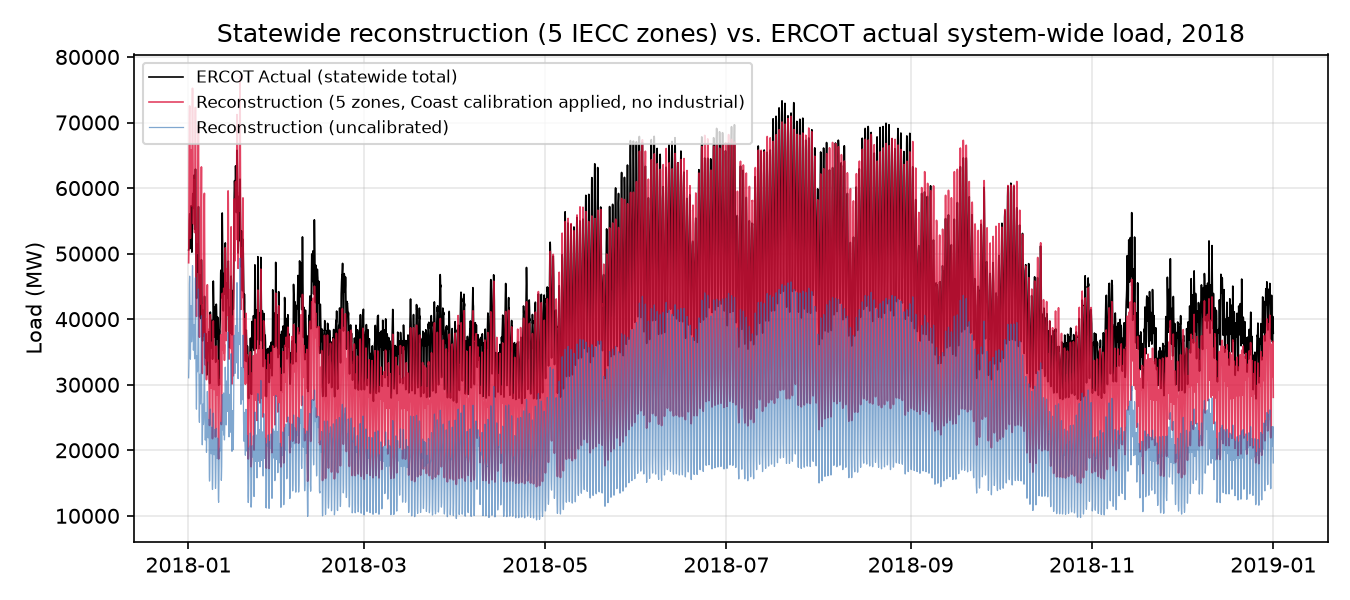
\includegraphics[width=0.85\textwidth]{figures/statewide_vs_ercot_fig1.png}
\caption{Statewide reconstruction (five IECC zones, residential + commercial) vs.\
ERCOT's actual statewide total load, 2018.}
\label{fig:global}
\end{figure}

\begin{table}[H]
\centering
\small
\begin{tabular}{lcc}
\toprule
& Peak (MW) & Pearson \\
\midrule
ERCOT actual, statewide total & 73{,}308.2 & --- \\
Reconstruction, uncalibrated, no industrial & 49{,}197.6 \;(67.1\%) & 0.9223 \\
Reconstruction, Coast calibration applied (speculative) & 76{,}856.9 \;($+4.8\%$) & 0.9231 \\
\bottomrule
\end{tabular}
\caption{The statewide aggregate correlates \emph{more strongly} with ERCOT's true
system total than any single zone does individually --- including Coast.}
\label{tab:global}
\end{table}

This is a genuinely new result, not merely a rescaled version of an existing one: the
statewide correlation (0.922) exceeds both Coast's own (0.90, Section~\ref{sec:recalibration})
and zone 3B's (0.71, Section~\ref{sec:ercot-crosswalk}). The most plausible explanation
is a diversity/smoothing effect --- summing five climatically distinct zones averages out
each zone's idiosyncratic noise and peak-timing offsets, directly analogous to the
coincidence/diversity-factor concept already used for review point 5
(Section~\ref{sec:validation}), just observed here at the statewide scale instead of
within one zone. Applying Coast's calibration factors statewide, despite having no
independent evidence they generalize (and zone 3B's much weaker local fit suggests they
may not, zone-by-zone), still lands within 5\% of ERCOT's true statewide peak --- a
reassuring, if speculative, consistency check. This result should be reported as
directional: there is still no independently-validated statewide calibration, and no
industrial model anywhere outside Coast's flat placeholder.

\emph{Both gaps are closed in Section~\ref{sec:zonecal}, which fits a calibration and a
data-driven industrial constant per ERCOT zone. Note also that the last row above is
more serious than it first appears: Coast's factors reach 105\% of the true peak
\emph{with no industrial load included at all}, which is what motivated abandoning them
as a statewide calibration.}

\section{Spatial Allocation Refinement: From Nearest-Bus to Area-Split}
\label{sec:areasplit}

Every result up to this point rested on a winner-takes-all spatial join: each census
tract gave \emph{all} of its dwellings to the single nearest bus, and each ZCTA gave
\emph{all} of its commercial floor space to the single nearest bus. This is the
spatial-assignment limitation the paper lists as future work, and it is the dominant
source of bus-level error --- not the load models, which by then were already validated.
Two new GIS exports replace it.

\subsection{Method}

Each 2020 census tract is subdivided into \textbf{50 equal-area parts}, and each 2010
ZCTA into \textbf{100 equal-area parts}; every part is then spatially joined to its own
nearest bus. The allocation weight follows directly:
\[
w(\text{polygon}, \text{bus}) \;=\; \frac{\text{parts won by that bus}}{\text{total parts}},
\]
in 2\% increments for tracts and 1\% for ZCTAs. A polygon's dwellings and floor space
are then distributed as a weighted sum over every bus that serves part of it, rather
than dumped on one. The subdivision was verified rather than assumed: within a tract
the 50 \texttt{Shape\_Area} values agree to $10^{-6}$ and sum to \texttt{ALAND}; within a
ZCTA the 100 values agree to $10^{-7}$.

A third export, \texttt{texas7k\_bus\_with\_climate\_zone.csv}, supplies the authoritative
bus table: all \textbf{6{,}717} Texas 7k buses with substation coordinates, nominal kV,
the case's own \texttt{Load\_MW}/\texttt{Gen\_MW}, county FIPS, IECC zone, and the ERCOT
\texttt{Area\_Name}. Previously a bus existed in the pipeline only if some tract had
chosen it (3{,}426 did), and its climate zone had to be inferred by majority vote over
those tracts. Two independent checks fall out of it: the file's own IECC zone agrees
with the NREL-derived county crosswalk on \textbf{100\% of 6{,}717 buses}, and
\texttt{Load\_MW} provides, for the first time, a per-bus reference against which a
\emph{spatial} allocation can be scored --- something no aggregate ERCOT comparison can do.

\subsection{Results}

Weights sum to one per polygon by construction, so the allocation is conservative:
\textbf{100.00\% of Texas housing units} (11{,}628{,}419) are retained, none
double-counted. Coverage and spatial agreement both improve substantially.

\begin{table}[H]
\centering
\small
\begin{tabular}{lcc}
\toprule
& Nearest-bus join & Area-split \\
\midrule
\multicolumn{3}{l}{\emph{Residential (50 parts per tract)}}\\
\quad Tracts split across $>$1 bus & 0\% & 84.0\% \\
\quad Buses receiving dwellings & 3{,}426 & \textbf{6{,}352} \\
\quad Load-carrying buses with zero dwellings & 1{,}824 & \textbf{25} \\
\quad Spearman $\rho$ vs.\ bus \texttt{Load\_MW} & 0.502 & \textbf{0.606} \\
\midrule
\multicolumn{3}{l}{\emph{Commercial (100 parts per ZCTA)}}\\
\quad ZCTAs split across $>$1 bus & 0\% & 90.2\% \\
\quad Buses receiving floor space & 1{,}598 & \textbf{6{,}329} \\
\quad Load-carrying buses with commercial load & 20.1\% & \textbf{96.1\%} \\
\quad Spearman $\rho$ vs.\ bus \texttt{Load\_MW} & 0.133 & \textbf{0.475} \\
\bottomrule
\end{tabular}
\caption{Effect of the area-split allocation, scored against the Texas 7k case's own
per-bus \texttt{Load\_MW}. Spearman (rank) rather than Pearson is the meaningful
statistic here: \texttt{Load\_MW} also contains industrial demand, so a handful of very
large industrial buses dominate any linear correlation.}
\label{tab:areasplit}
\end{table}

\begin{figure}[H]
\centering
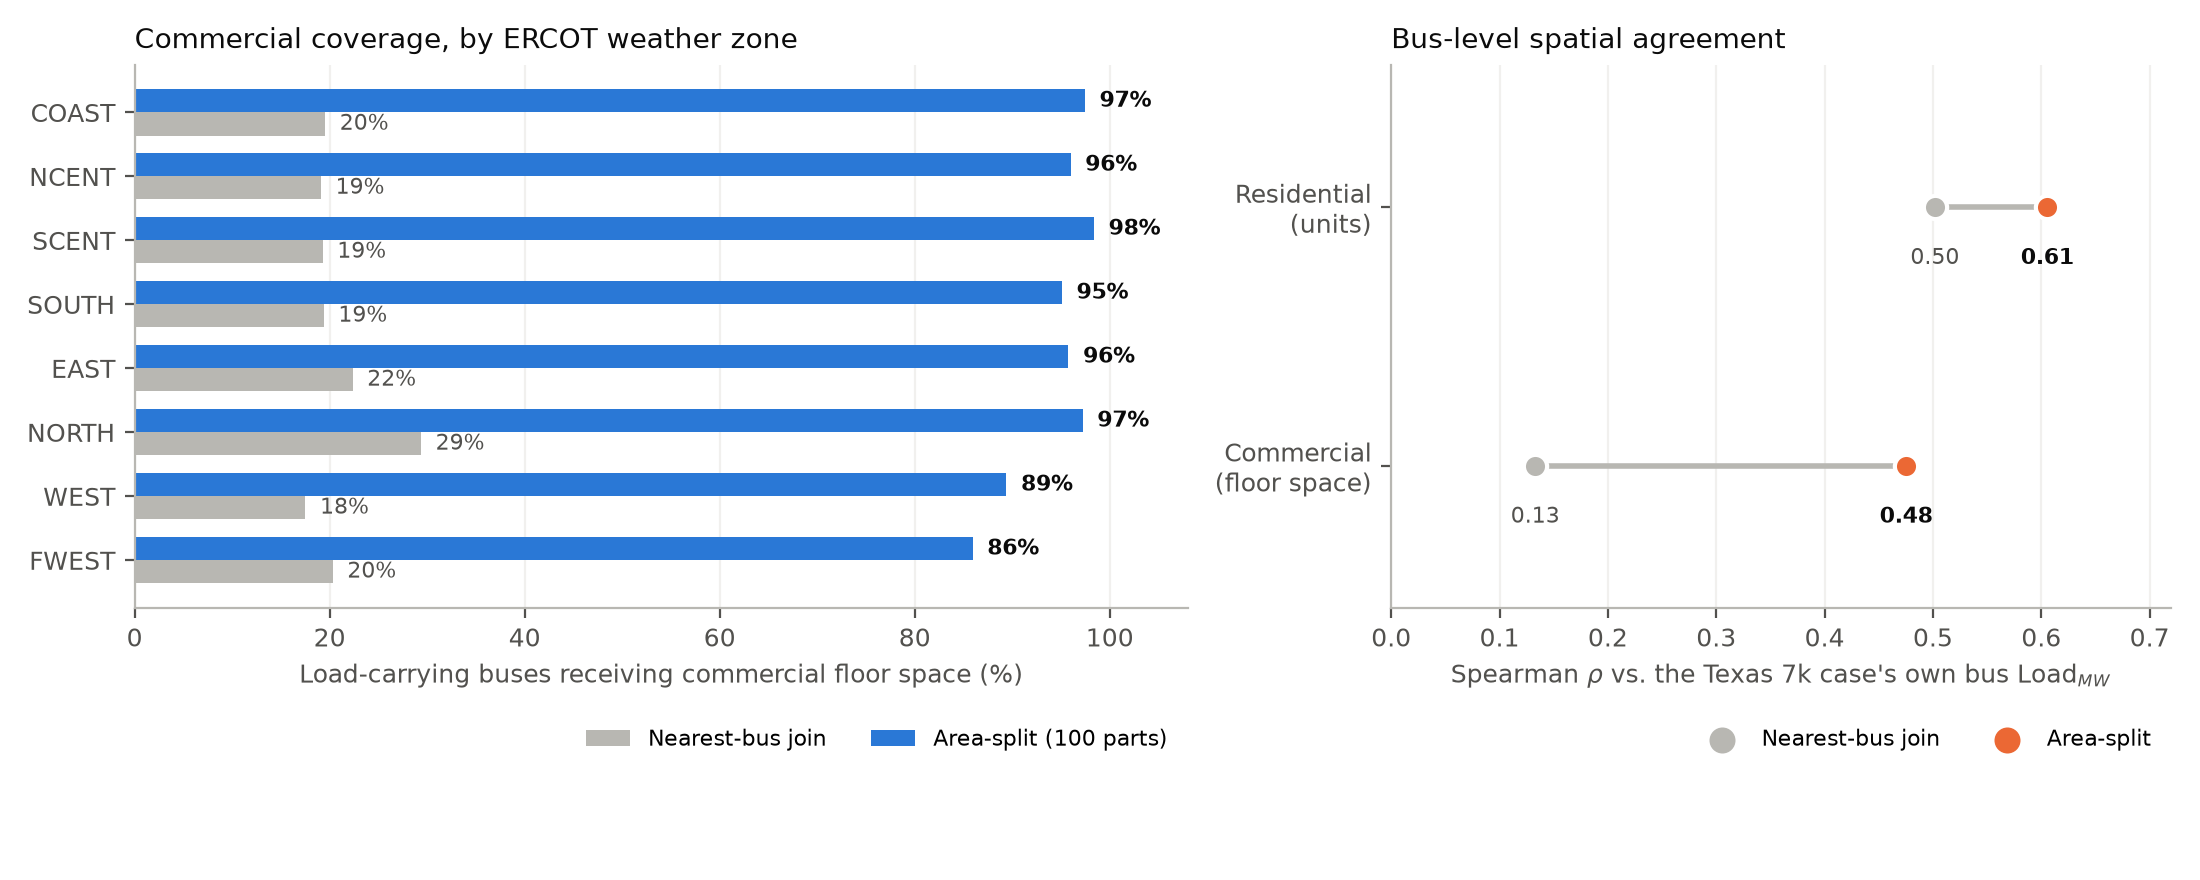
\includegraphics[width=\textwidth]{figures/area_split_fig1.png}
\caption{Left: share of load-carrying buses receiving commercial floor space, by ERCOT
weather zone. Right: bus-level rank agreement with the case's own \texttt{Load\_MW}.}
\label{fig:areasplit}
\end{figure}

The commercial gain is the larger one, because the nearest-ZCTA join was the more
degenerate of the two: with only 2{,}031 ZCTAs to distribute over 6{,}717 buses, just
1{,}598 buses (23.8\%) could ever receive commercial load at all, in any zone --- and only
20.1\% of the buses that actually carry load in the grid case.

\subsection{A Negative Result Worth Recording}

The area split was expected to also repair a degenerate per-zone commercial calibration
(Section~\ref{sec:zonecal}, where South Central fits $\mathrm{COM\_SCALE}=0$). \textbf{It
did not}, and the reason is structural rather than empirical: redistributing floor space
\emph{among buses of the same ERCOT zone} leaves that zone's aggregate unchanged (zone
totals moved by $-1.6\%$ to $+7.8\%$, most under 2\%), and the calibration is fitted on
the aggregate. Every zone-level validation number in Sections~\ref{sec:ercot8} and
\ref{sec:zonecal} is, to three decimals, what it was before the ZCTA export landed.

This is worth stating plainly in the paper: the area split is a \emph{bus-level}
improvement, and bus-level fidelity is what the framework exists to produce, but it is
invisible to any zone-aggregate metric. It is precisely the kind of improvement that a
validation protocol based only on aggregate correlation would fail to detect --- which is
itself an argument for reporting the \texttt{Load\_MW} rank statistic above.

\section{ERCOT Weather-Zone Validation: All Eight Zones}
\label{sec:ercot8}

Section~\ref{sec:ercot-crosswalk} validated a single IECC zone (3B) against a
county-to-ERCOT-weather-zone crosswalk read by eye from ERCOT's published picture map,
and stated that extending this to the remaining zones would require GIS shapefiles that
are not publicly available. \textbf{That obstacle is now removed}, from an unexpected
direction: the authoritative bus table carries an \texttt{Area\_Name} field holding
exactly ERCOT's eight weather-zone names. The crosswalk is therefore per bus, taken from
the grid model itself, with no county approximation and no map reading. The 3B result is
superseded by what follows and is retained above only as methodology history.

\subsection{Validating the Crosswalk Before Using It}

\texttt{Area\_Name} was checked before being trusted. The Texas 7k case is a peak-load
snapshot, so each area's summed \texttt{Load\_MW} should sit near that ERCOT zone's 2018
peak. Six of eight do; two clearly do not.

\begin{table}[H]
\centering
\small
\begin{tabular}{lccc}
\toprule
ERCOT zone & Case peak (MW) & ERCOT 2018 peak (MW) & Ratio \\
\midrule
COAST & 20{,}130.7 & 20{,}269.8 & 0.99 \\
FWEST & 3{,}558.9 & 3{,}655.0 & 0.97 \\
NCENT & 24{,}706.5 & 26{,}499.2 & 0.93 \\
SOUTH & 5{,}646.1 & 6{,}176.1 & 0.91 \\
WEST & 1{,}886.3 & 2{,}083.6 & 0.91 \\
SCENT & 11{,}899.7 & 14{,}166.7 & 0.84 \\
\midrule
EAST & 3{,}473.7 & 2{,}620.8 & \textbf{1.33} \\
NORTH & 3{,}364.7 & 1{,}521.8 & \textbf{2.21} \\
\midrule
Statewide & 74{,}666.6 & 73{,}308.2 & 1.02 \\
\bottomrule
\end{tabular}
\caption{The synthetic case's EAST and NORTH area boundaries do not coincide with
ERCOT's. Those two zones are reported throughout with a boundary-mismatch flag: their
shape statistics remain interpretable, their magnitude statistics do not.}
\label{tab:areacheck}
\end{table}

\subsection{Results}

The residential and commercial bus-level reconstructions from all five IECC zones are
concatenated and grouped by each bus's ERCOT zone --- an aggregation the previous
county-based approach could not express, since a single ERCOT zone such as SCENT draws
buses from IECC 2A and 3A at once.

\begin{table}[H]
\centering
\small
\begin{tabular}{lcccc}
\toprule
ERCOT zone & ERCOT peak (MW) & Recon.\ peak (MW) & Peak coverage & Pearson $r$ \\
\midrule
COAST & 20{,}269.8 & 13{,}233.6 & 65.3\% & 0.900 \\
NCENT & 26{,}499.2 & 17{,}000.0 & 64.2\% & 0.900 \\
SCENT & 14{,}166.7 & 9{,}039.0 & 63.8\% & 0.887 \\
SOUTH & 6{,}176.1 & 3{,}993.7 & 64.7\% & 0.909 \\
WEST & 2{,}083.6 & 914.5 & 43.9\% & 0.815 \\
FWEST & 3{,}655.0 & 2{,}299.7 & 62.9\% & \textbf{0.629} \\
EAST$^\dagger$ & 2{,}620.8 & 3{,}494.2 & --- & 0.911 \\
NORTH$^\dagger$ & 1{,}521.8 & 1{,}730.6 & --- & 0.905 \\
\midrule
\textbf{ERCOT total} & 73{,}308.2 & 49{,}197.6 & 67.1\% & \textbf{0.922} \\
\bottomrule
\end{tabular}
\caption{Uncalibrated reconstruction (no scale factors, no industrial model) against
ERCOT actual load, 2018. $^\dagger$ boundary mismatch: peak coverage is not meaningful
for these two zones.}
\label{tab:ercot8}
\end{table}

Three findings. First, the framework holds up across climatically distinct regions:
four of the six well-matched zones (COAST, NCENT, SCENT, SOUTH) land between $r=0.887$
and $r=0.909$. Uncalibrated peak coverage is more uniform still --- five of the six sit
between 62.9\% and 65.3\%, WEST being the sole exception at 43.9\% --- and that
consistency suggests one systematic missing component rather than per-zone modeling
noise.

Second, the statewide aggregate ($r=0.922$) again exceeds every individual zone, the
diversity/smoothing effect already reported in Section~\ref{sec:global}, now measured
against a correctly-partitioned set of zones rather than an approximate one.

Third, \textbf{FWEST is the clear outlier} ($r=0.629$), with WEST second ($r=0.815$).
This confirms, far more precisely than the earlier county-approximated 3B result
($r=0.71$ over a hand-built 67-county subset), that the weakness is specific to West
Texas and the Permian Basin rather than a general property of drier climate zones.

\section{Per-Zone Calibration with a Fitted Industrial Constant}
\label{sec:zonecal}

Coast's recalibrated factors (Section~\ref{sec:recalibration}: $\mathrm{RES\_SCALE}=1.6$,
$\mathrm{COM\_SCALE}=1.3$, plus a hand-picked flat 4{,}500\,MW industrial term) were fitted
on Coast alone. A direct test shows they do not transfer: applied statewide
\emph{with no industrial term at all}, they already reach 76{,}857\,MW, or \textbf{105\%
of ERCOT's true statewide peak}. The residential scale factor had evidently been
absorbing missing industrial demand.

\subsection{Method}

Each ERCOT zone is calibrated independently under
\[
\mathrm{ERCOT}_z(t) \;=\; \mathrm{RES}_z \cdot r_z(t) \;+\; \mathrm{COM}_z \cdot c_z(t) \;+\; \mathrm{IND}_z ,
\]
solved by non-negative least squares. Two departures from the Coast method matter. The
industrial term is \textbf{fitted rather than assumed}, making $\mathrm{IND}_z$ a
data-driven estimate of each zone's weather-insensitive baseload; and the fit is scored
by \textbf{blocked seasonal 4-fold cross-validation} (fit on three seasons, score on the
held-out one), the same protocol used for the load models throughout this report. A
calibration fitted and scored on the same 8{,}760 hours would be optimistic in precisely
the way diagnosed in Section~\ref{sec:temporal}.

Collinearity was checked before interpreting any individual coefficient: on
centered-and-scaled columns the design matrix has condition number $\approx 2.3$ and
VIF $\approx 1.9$, so the residential/commercial split is well posed.

\subsection{Results}

\begin{table}[H]
\centering
\small
\begin{tabular}{lccccc}
\toprule
ERCOT zone & RES & COM & IND (MW) & CV MAE (MW) & Pearson $r$ \\
\midrule
COAST & 1.07 & 0.98 & 5{,}594 & 1{,}105 \;(from 1{,}933) & 0.900 \\
NCENT & 1.36 & 0.98 & 4{,}863 & 1{,}496 \;(from 1{,}884) & 0.901 \\
SCENT & 1.26 & \textbf{0.00} & 2{,}531 & 715 \;(from 1{,}002) & 0.902 \\
SOUTH & 1.14 & 0.66 & 1{,}541 & 304 \;(from 578) & 0.911 \\
WEST & 1.07 & \textbf{3.03} & 692 & 124 \;(from 227) & 0.823 \\
FWEST & \textbf{0.30} & 1.46 & 2{,}236 & 213 \;(from 602) & 0.655 \\
EAST$^\dagger$ & 0.58 & 0.70 & 642 & 122 \;(from 223) & 0.911 \\
NORTH$^\dagger$ & 0.58 & 0.77 & 393 & 69 \;(from 125) & 0.905 \\
\midrule
\textbf{ERCOT total} & \textbf{1.15} & \textbf{0.76} & \textbf{18{,}079} & \textbf{3{,}462} \;(from 6{,}085) & \textbf{0.924} \\
\bottomrule
\end{tabular}
\caption{Per-zone calibration. ``from'' gives the blocked-seasonal-CV MAE of the
Coast-style two-parameter fit with no industrial term, for comparison.
$^\dagger$ boundary mismatch, reported for completeness.}
\label{tab:zonecal}
\end{table}

\begin{figure}[H]
\centering
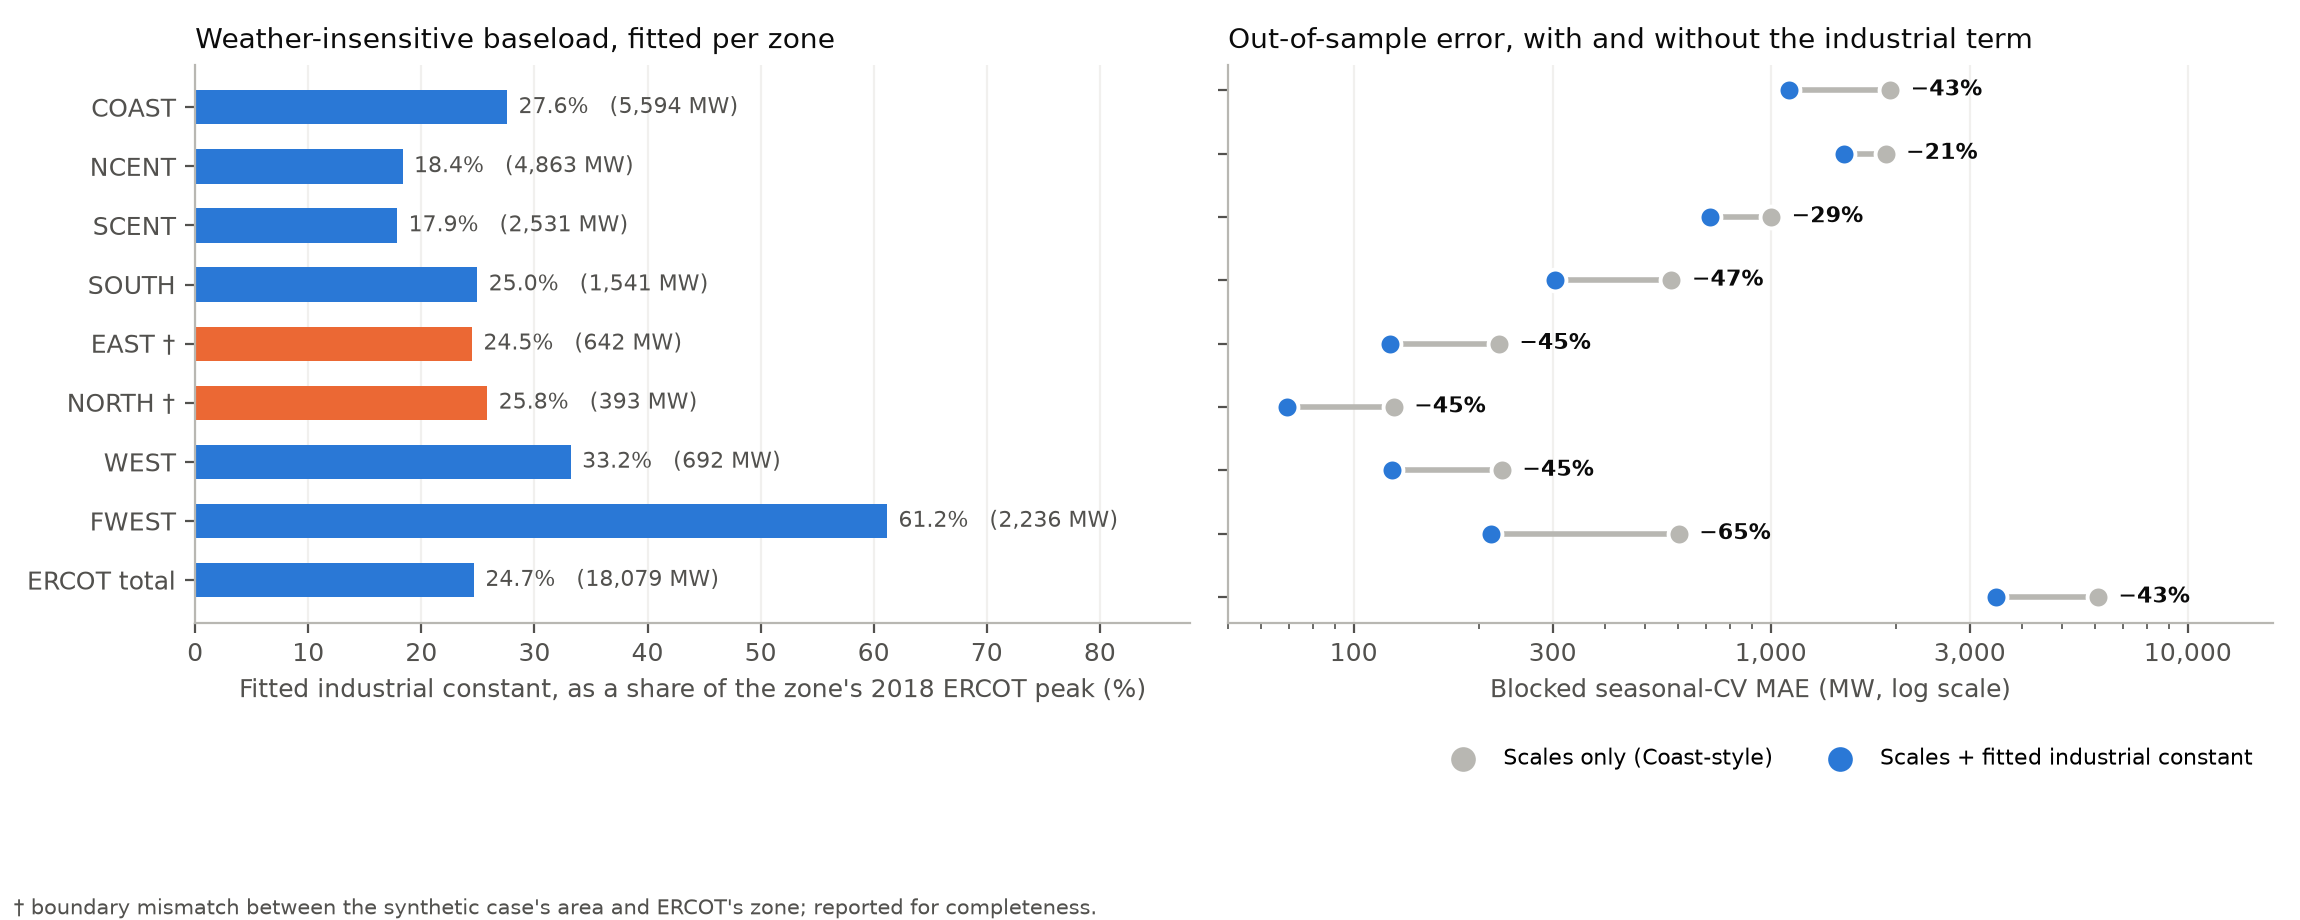
\includegraphics[width=\textwidth]{figures/zone_calibration_fig1.png}
\caption{Left: the fitted weather-insensitive baseload as a share of each zone's ERCOT
peak. Right: out-of-sample error with and without the industrial term.}
\label{fig:zonecal}
\end{figure}

\begin{figure}[H]
\centering
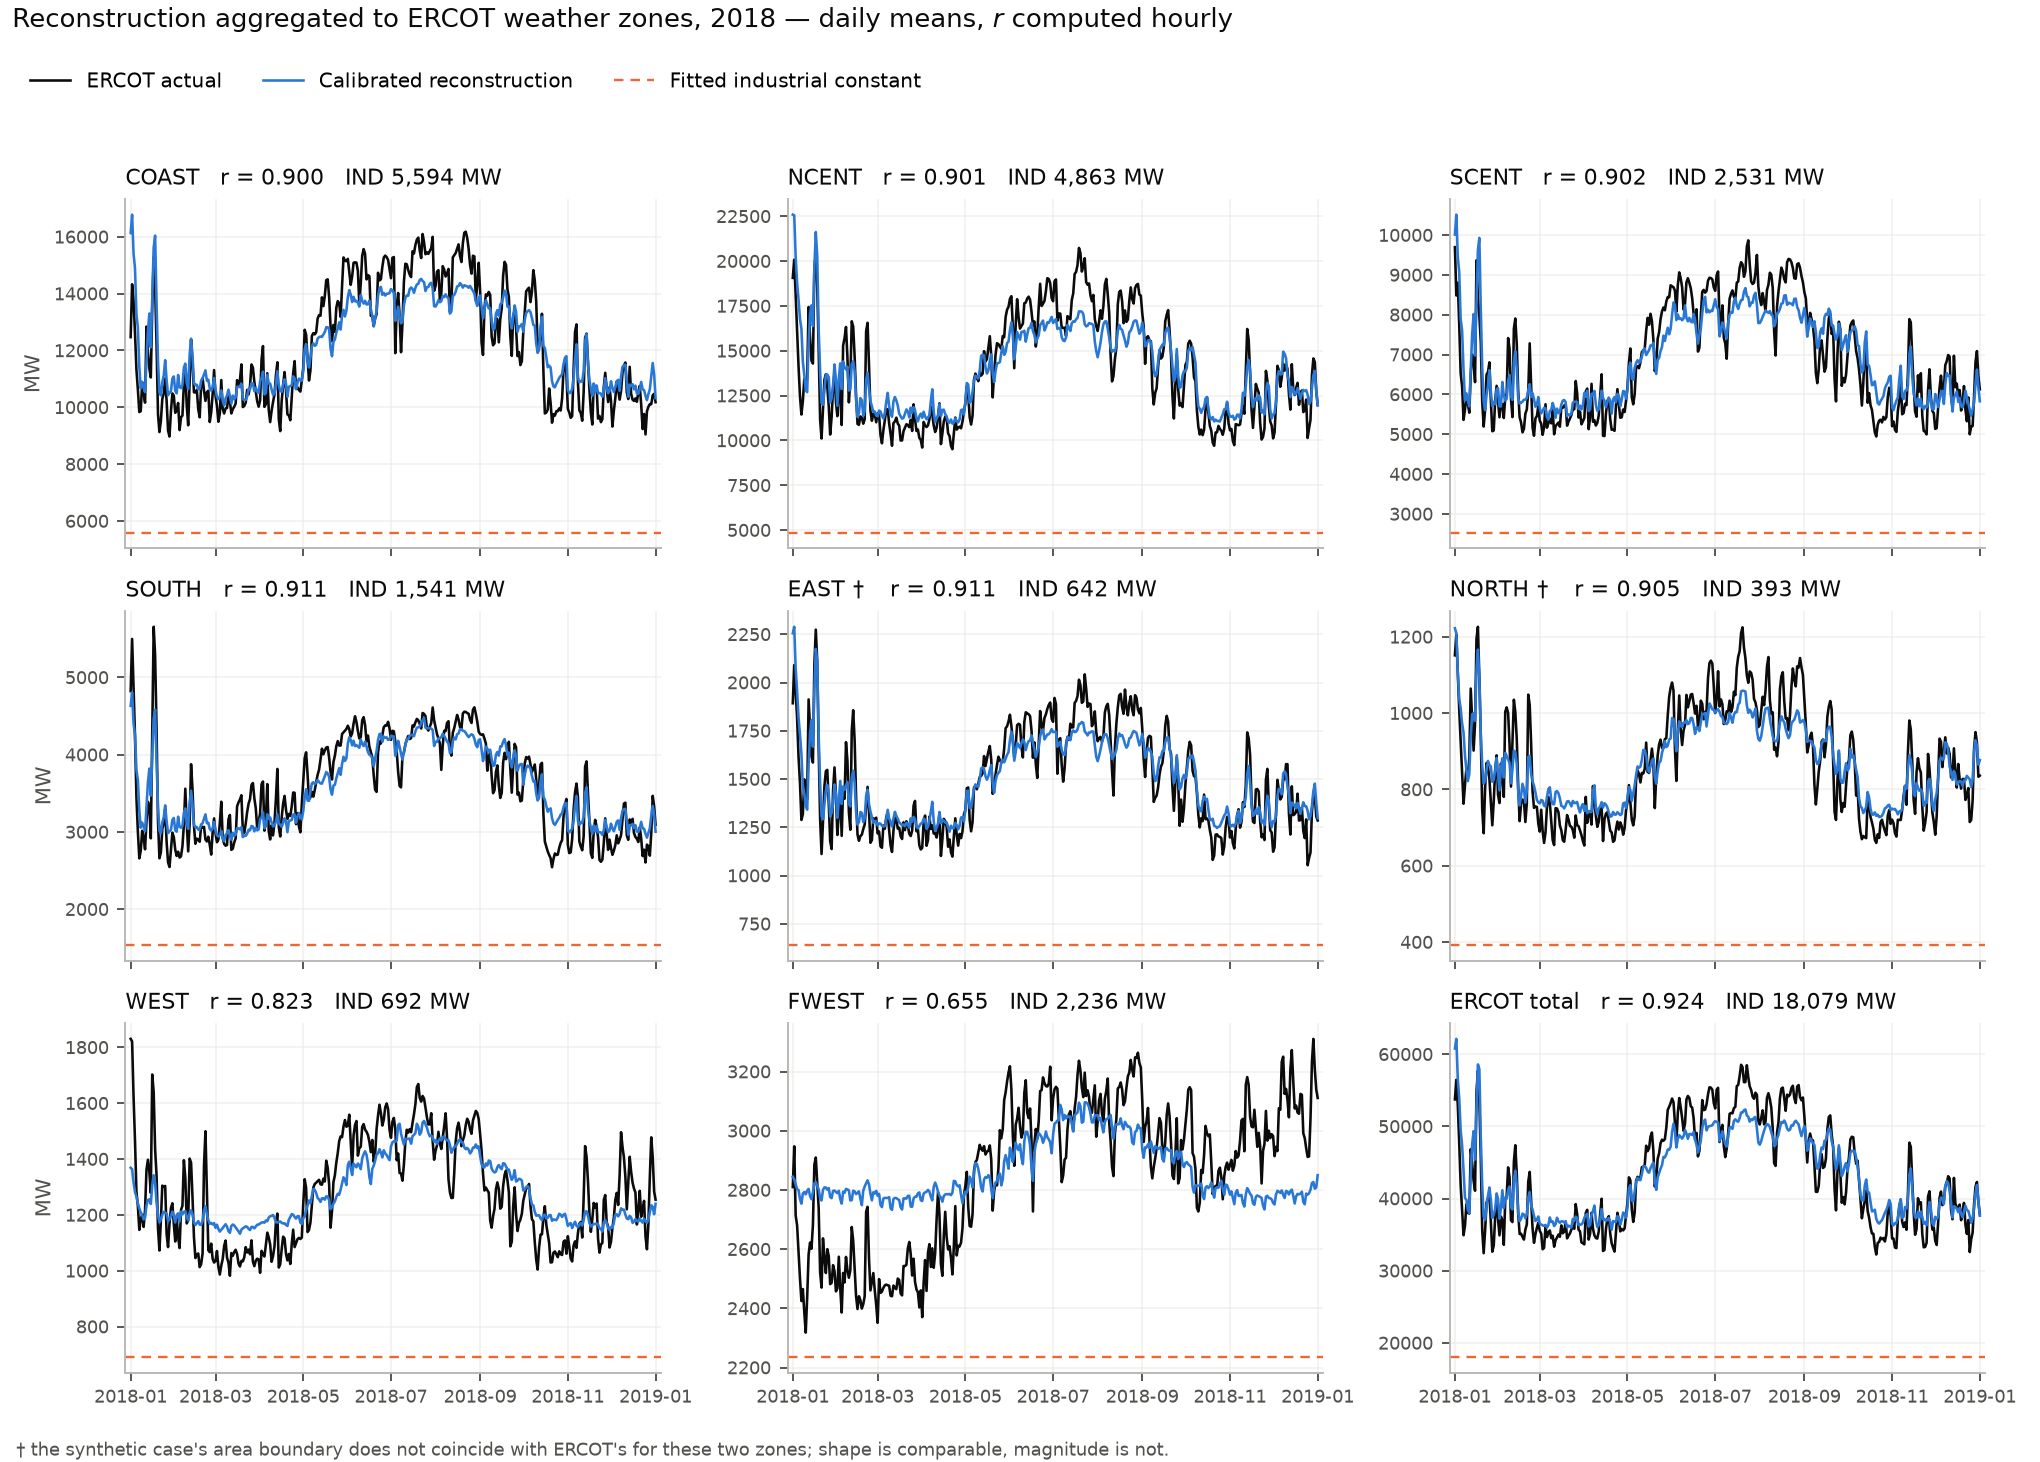
\includegraphics[width=\textwidth]{figures/ercot_8zone_fig1.png}
\caption{Calibrated bus-level reconstruction aggregated to each ERCOT weather zone,
2018. Daily means are plotted for legibility; the reported $r$ is computed on hourly
data.}
\label{fig:ercot8}
\end{figure}

Four results stand out.

\textbf{The building-stock reconstruction barely needs a fudge factor.} Once an
industrial term is present, $\mathrm{RES}$ falls to 1.07--1.36 in five of the six
well-matched zones (FWEST, at 0.30, is the exception discussed below), against 1.6--1.9
for Coast without one. This is a meaningful argument for the
method: the earlier large scale factors were compensating for a missing load component,
not for a mis-sized housing stock.

\textbf{Industrial demand is roughly a quarter of ERCOT.} The statewide fit puts it at
18{,}079\,MW, or 24.7\% of the system peak. Coast alone fits 5{,}594\,MW, which
retrospectively validates the paper's hand-picked 4{,}500\,MW placeholder as the right
order of magnitude and slightly low.

\textbf{FWEST is structurally industrial.} It fits $\mathrm{RES}=0.30$ and an industrial
constant equal to \textbf{61.2\% of its peak} --- by far the highest share of any zone, and
a quantitative explanation for its weak correlation. Its load is mostly not a function
of weather, so no weather-driven reconstruction can track it.

\textbf{Out-of-sample error drops sharply}, by 21\% (NCENT) to 65\% (FWEST) per zone,
and by 43\% statewide (blocked-seasonal-CV MAE 6{,}085 $\rightarrow$ 3{,}462\,MW).

\subsection{Two Caveats, One Unresolved}

A constant added to an \emph{already-fixed} prediction cannot change a correlation, since
$\mathrm{corr}(y, ax+b)$ does not depend on $b$. Here $\mathrm{IND}$ is fitted
\emph{jointly} with the scales, which does move the shape slightly --- without an
industrial term the scales are forced upward to reach the right level, distorting the
residential/commercial mix. The effect is real but small (FWEST $0.631\rightarrow0.655$,
WEST $0.807\rightarrow0.823$, every other zone $+0.002$). The industrial constant should
therefore be reported as a magnitude correction, not as a fix for the weak-shape zones.

Two coefficients remain anomalous: SCENT fits $\mathrm{COM\_SCALE}=0.00$ and WEST fits
3.03. The obvious explanation --- poor commercial bus coverage --- was tested and rejected
(Section~\ref{sec:areasplit}). The real diagnosis, for SCENT, is that the
\emph{partial} correlation of the commercial profile with ERCOT load, with residential
removed, is $-0.014$, against $+0.24$ to $+0.34$ in every other zone: the commercial
stack genuinely adds no information there beyond residential plus a constant. Why this
should be true of the Austin/San~Antonio corridor specifically is \textbf{not yet
explained}, and is flagged as an open item rather than resolved.

\section{Open Items and Next Steps}
\label{sec:nextsteps}

\begin{itemize}
    \item \textbf{RES\_SCALE/COM\_SCALE recalibration --- DONE (Section~\ref{sec:recalibration}).}
    New calibration RES\_SCALE=1.6, COM\_SCALE=1.3, roughly halving the absolute error
    (MAE 2{,}117\,MW $\rightarrow$ 1{,}201\,MW) against the current best pipeline.
    \item \textbf{Extension to all of Texas --- DONE (Section~\ref{sec:statewide}).}
    The missing bus-to-load spatial mapping has since been obtained for both residential
    and commercial, and subsequently replaced by the full 6{,}717-bus authoritative table
    with an area-split allocation (Section~\ref{sec:areasplit}). All five IECC
    zones now have honest R\textsuperscript{2} results and are cross-checked against
    Coast at $r>0.996$.
    \item \textbf{Weekday/weekend breakdown of residential R\textsuperscript{2}}:
    Section~\ref{sec:validation} shows the winter-weekend diurnal-shape correlation
    is the single weakest metric in this report, and that it was fixed by the weather
    correction specifically, not by later refinements. A direct weekday/weekend
    breakdown of the seasonal-CV R\textsuperscript{2} itself (rather than only the
    aggregate shape correlation) has not yet been produced. Still not done; now also
    an open question for the four other statewide zones.
    \item \textbf{Comparison against prior proportional allocation methods}
    (review point 9, ``Hanyue's method''): still blocked on obtaining the method
    reference itself.
    \item \textbf{Spatial diversity between buses}: all buses within a zone still
    share a single, zone-wide blended weather series (Section~\ref{sec:weather}).
    Still not implemented; the statewide extension makes this a bigger question, since
    a 79-county zone-wide blend (2A) dilutes local signal more than Coast's original
    12-county blend did (quantified in the $\sim$5\% cross-check gap,
    Table~\ref{tab:crosscheck}).
    \item \textbf{Commercial bus-coverage gap --- DONE (Section~\ref{sec:areasplit}).}
    The nearest-ZCTA join left four buses in five unable to receive any commercial load.
    An area-split join (100 equal-area parts per ZCTA, each matched to its nearest bus)
    raises coverage of load-carrying buses from 20.1\% to 96.1\% and rank agreement with
    the case's own \texttt{Load\_MW} from $\rho=0.133$ to $0.475$. The equivalent split
    for tracts (50 parts) cut load-carrying buses with zero dwellings from 1{,}824 to 25.
    \item \textbf{Industrial load, statewide --- PARTIALLY ADDRESSED
    (Section~\ref{sec:zonecal}).} Each ERCOT zone now carries a \emph{fitted}
    weather-insensitive constant instead of a hand-picked one, totalling 18{,}079\,MW
    statewide (24.7\% of system peak), which roughly halves out-of-sample error. But a
    constant is still not a model: it cannot reproduce industrial load's own temporal
    variation, which is precisely what FWEST needs ($r=0.629$, with a fitted constant
    equal to 61.2\% of its peak). A genuinely time-varying, data-driven industrial
    representation remains the single most consequential open item.
    \item \textbf{ERCOT weather-zone crosswalk --- DONE (Section~\ref{sec:ercot8}).}
    No shapefiles were needed in the end: the grid model's own \texttt{Area\_Name}
    field assigns every bus to an ERCOT weather zone. All eight zones plus the ERCOT
    total now have a real validation number.
    \item \textbf{EAST and NORTH boundary mismatch (NEW,
    Section~\ref{sec:ercot8}):} the synthetic case's area load for these two zones is
    1.33$\times$ and 2.21$\times$ their ERCOT peak, so the case's boundaries there do not
    coincide with ERCOT's. Their shape statistics are reported, their magnitudes are
    not. Diagnosing which counties are misassigned would make two more zones fully
    usable; not attempted.
    \item \textbf{South Central's null commercial coefficient (NEW,
    Section~\ref{sec:zonecal}):} SCENT fits $\mathrm{COM\_SCALE}=0$, and the partial
    correlation of its commercial profile with ERCOT load (residential removed) is
    $-0.014$, against $+0.24$ to $+0.34$ everywhere else. Coverage and collinearity were
    both tested and rejected as explanations. Unexplained; isolated to the
    Austin/San~Antonio corridor.
    \item \textbf{Model choice for the paper}: Section~\ref{sec:models} supports
    either retaining RandomForest (simpler, statistically equivalent system-level
    result) or adopting LightGBM (materially better per-archetype accuracy at zero
    system-level cost). The statewide extension (Section~\ref{sec:statewide}) used
    LightGBM throughout, so this is effectively the working default now, but the
    framing decision for the paper text itself is still open.
\end{itemize}

\subsection{What Would Help This Move Faster}
\label{sec:asks}

\begin{itemize}
    \item \textbf{Real ERCOT weather-zone GIS shapefiles --- no longer needed.}
    Previously listed here as the single highest-leverage missing input; the grid
    model's \texttt{Area\_Name} field supplied the assignment instead
    (Section~\ref{sec:ercot8}). Retained here only to record that the ask is closed.
    \item \textbf{A data source and methodology for industrial load}, statewide ---
    now with a target to hit. Section~\ref{sec:zonecal} quantifies how much
    weather-insensitive load each zone is missing (18{,}079\,MW statewide; 61.2\% of
    peak in FWEST against 17.9\% in SCENT), which confirms that industrial share varies
    enormously by region and gives any candidate industrial dataset a per-zone number
    to be checked against.
    \item \textbf{The Hanyue proportional-allocation method reference} (review point 9),
    to unblock the one remaining unimplemented item from the point-5 validation work.
    \item \textbf{A decision on scope for the paper}: whether the
    statewide extension (Sections~\ref{sec:statewide}--\ref{sec:global}) belongs in
    the current submission as an additional contribution, or is better positioned as
    follow-up work referenced briefly --- this materially changes how much of the above
    needs to be resolved before submission versus after.
\end{itemize}

\section{Conclusion}

Two independent, previously undiagnosed issues in the original pipeline --- temporal
train/test leakage and an incorrect weather station geography --- were identified, root-
caused, and corrected under a single, consistent, honest evaluation protocol (blocked
seasonal 4-fold cross-validation). Both corrections improved, rather than hurt, the
paper's headline system-level validation metric (Pearson correlation against ERCOT
Coast actual load), while substantially lowering the previously-inflated per-archetype
R\textsuperscript{2} figures to their honest values. A model comparison
(RandomForest/XGBoost/LightGBM) and a feature-engineering ablation study, both run
through the same protocol, directly address review points 5 and 6: model choice
improves per-archetype accuracy but not the system-level number, while a cheap
lag-temperature feature addition improves both. A final full comparison across all
six pipeline versions (Section~\ref{sec:validation}) shows this improvement is not
perfectly uniform across every secondary metric --- the temporal and weather fixes did
most of the work on shape-sensitive metrics like the winter-weekend diurnal
correlation, while model choice and feature engineering mainly improved accuracy and
the headline correlation. The corrected, feature-engineered LightGBM pipeline is
recommended as the version to report in the paper going forward.

This corrected pipeline was then extended from the single Coast case study to all five
Texas IECC climate zones (Section~\ref{sec:statewide}), reusing the exact
methodology validated on Coast, and cross-checked against it at $r>0.996$ on both the
residential and commercial stacks. The Coast calibration itself was found to be stale
and was refreshed (Section~\ref{sec:recalibration}), materially reducing absolute
error.

Three further results complete the picture. First, the winner-takes-all spatial join
that underpinned every earlier number --- one tract, one bus --- was replaced by an
area-split allocation (Section~\ref{sec:areasplit}), conserving 100\% of Texas housing
units while raising the share of load-carrying buses that receive commercial load from
20\% to 96\% and roughly quadrupling bus-level rank agreement with the grid case's own
per-bus load. Notably, this improvement is invisible to every zone-aggregate metric in
this report, which is itself an argument for reporting a bus-level statistic.

Second, validation was extended from one hand-crosswalked zone to \emph{all eight} ERCOT
weather zones (Section~\ref{sec:ercot8}), using a per-bus assignment carried by the grid
model itself rather than the unobtainable GIS shapefiles previously assumed necessary.
Four of the six well-matched zones fall between $r=0.887$ and $r=0.909$, five of the six
show uncalibrated peak coverage within 62.9--65.3\%, and the statewide aggregate again
leads at $r=0.922$. The earlier zone-3B finding is reproduced and sharpened: the weakness is
specific to West Texas ($r=0.629$ for FWEST), not to dry climates generally.

Third, calibration was refitted per zone with a \emph{data-driven} industrial constant
(Section~\ref{sec:zonecal}), scored out-of-sample by the same blocked seasonal protocol.
Coast's factors were shown not to transfer --- applied statewide with no industrial term
they already reach 105\% of ERCOT's true peak --- while the refitted residential scale
factors collapse to 1.07--1.36 in five of the six well-matched zones, indicating that the
earlier large factors were standing in for missing industrial demand rather than
correcting the housing stock. That missing
demand is now quantified at 18{,}079\,MW statewide, 24.7\% of system peak, and out-of-sample
error roughly halves.

Together, these results show the framework generalizes well beyond its original
single-zone case study, while being explicit about where it does not yet hold: industrial
load is a fitted constant rather than a model, and a constant cannot rescue the one zone
that most needs it (FWEST, whose weather-insensitive share is 61\% of peak); two ERCOT
zones (EAST, NORTH) have boundary mismatches that make their magnitudes uninterpretable;
and South Central's null commercial coefficient remains unexplained after coverage and
collinearity were both tested and ruled out. Section~\ref{sec:asks} lists what would most
efficiently close the remaining gaps.

\end{document}
